\documentclass[a4paper]{article}\usepackage[]{graphicx}\usepackage[]{color}
% maxwidth is the original width if it is less than linewidth
% otherwise use linewidth (to make sure the graphics do not exceed the margin)
\makeatletter
\def\maxwidth{ %
  \ifdim\Gin@nat@width>\linewidth
    \linewidth
  \else
    \Gin@nat@width
  \fi
}
\makeatother

\definecolor{fgcolor}{rgb}{0.345, 0.345, 0.345}
\makeatletter
\@ifundefined{AddToHook}{}{\AddToHook{package/xcolor/after}{\definecolor{fgcolor}{rgb}{0.345, 0.345, 0.345}}}
\makeatother
\newcommand{\hlnum}[1]{\textcolor[rgb]{0.686,0.059,0.569}{#1}}%
\newcommand{\hlstr}[1]{\textcolor[rgb]{0.192,0.494,0.8}{#1}}%
\newcommand{\hlcom}[1]{\textcolor[rgb]{0.678,0.584,0.686}{\textit{#1}}}%
\newcommand{\hlopt}[1]{\textcolor[rgb]{0,0,0}{#1}}%
\newcommand{\hlstd}[1]{\textcolor[rgb]{0.345,0.345,0.345}{#1}}%
\newcommand{\hlkwa}[1]{\textcolor[rgb]{0.161,0.373,0.58}{\textbf{#1}}}%
\newcommand{\hlkwb}[1]{\textcolor[rgb]{0.69,0.353,0.396}{#1}}%
\newcommand{\hlkwc}[1]{\textcolor[rgb]{0.333,0.667,0.333}{#1}}%
\newcommand{\hlkwd}[1]{\textcolor[rgb]{0.737,0.353,0.396}{\textbf{#1}}}%
\let\hlipl\hlkwb

\usepackage{framed}
\makeatletter
\newenvironment{kframe}{%
 \def\at@end@of@kframe{}%
 \ifinner\ifhmode%
  \def\at@end@of@kframe{\end{minipage}}%
  \begin{minipage}{\columnwidth}%
 \fi\fi%
 \def\FrameCommand##1{\hskip\@totalleftmargin \hskip-\fboxsep
 \colorbox{shadecolor}{##1}\hskip-\fboxsep
     % There is no \\@totalrightmargin, so:
     \hskip-\linewidth \hskip-\@totalleftmargin \hskip\columnwidth}%
 \MakeFramed {\advance\hsize-\width
   \@totalleftmargin\z@ \linewidth\hsize
   \@setminipage}}%
 {\par\unskip\endMakeFramed%
 \at@end@of@kframe}
\makeatother

\definecolor{shadecolor}{rgb}{.97, .97, .97}
\definecolor{messagecolor}{rgb}{0, 0, 0}
\definecolor{warningcolor}{rgb}{1, 0, 1}
\definecolor{errorcolor}{rgb}{1, 0, 0}
\makeatletter
\@ifundefined{AddToHook}{}{\AddToHook{package/xcolor/after}{
\definecolor{shadecolor}{rgb}{.97, .97, .97}
\definecolor{messagecolor}{rgb}{0, 0, 0}
\definecolor{warningcolor}{rgb}{1, 0, 1}
\definecolor{errorcolor}{rgb}{1, 0, 0}
}}
\makeatother
\newenvironment{knitrout}{}{} % an empty environment to be redefined in TeX

\usepackage{alltt}
\usepackage[american]{babel}
\usepackage[T1]{fontenc}
\usepackage[utf8]{inputenc}
\usepackage{tabulary}
\usepackage{tocloft}
\usepackage{relsize}
\usepackage{hyperref}
\usepackage{apacite}
\usepackage{geometry}
\geometry{verbose,tmargin=2cm,bmargin=2cm,lmargin=1.5cm,rmargin=1.5cm}

%-----  Customization & setup --------------------

\hypersetup{linktocpage}
\hypersetup{
    colorlinks,
    citecolor=black,
    filecolor=black,
    linkcolor=blue,
    urlcolor=blue
}
\renewcommand{\cftsecdotsep}{\cftdotsep}  % damit auch die Hauptsections im TOC Punkte zu den Seitenzahlen haben








% R ouput should be only 80 characters wide

%--------------------------------------------------	








\title{Round robin analyses in R: How to use TripleR}
\author{Felix D. Sch\"onbrodt\thanks{\copyright~\today,~Felix Sch\"onbrodt, Department of Psychology, Ludwig-Maximilians-University, Germany. This package partly was written during a Google Summer of Code 2010 project. Comments on this document may be sent to the author at felix@nicebread.de}
\and Stefan C. Schmukle\thanks{University of Leipzig, Germany}
\and Mitja D. Back\thanks{University of Münster, Germany}}
\IfFileExists{upquote.sty}{\usepackage{upquote}}{}
\begin{document}	
\maketitle
\tableofcontents
\setcounter{tocdepth}{2}
\clearpage

TripleR\footnote{When you use TripleR in your research, please cite it as Schönbrodt, F. D., Back, M. D.,  \& Schmukle, S. C. (2012). TripleR: An R package for social relations analyses based on round-robin designs. \emph{Behavior Research Methods, 44}, 455-470. doi:10.3758/s13428-011-0150-4
} provides functions with a simple, yet powerful interface to calculate round robin analyses in R. We assume that you are already familiar with social relations analyses. If not, a good starter would be David Kenny's website\footnote{http://davidakenny.net/kenny.htm}, or some introductory articles (e.g., \citeNP{Back2010}; \citeNP{Kenny2006}, \citeNP{Kenny_LaVoie_1984}; especially Ch. 8; \citeNP{Kenny1994}, for detailed description of the model and the formulae). 

If you have already done your round robin study, this document will explain how to get your data into the right format, how to tell TripleR what analyses to do, and how to work with the results. In social relations analyses (SRAs), two notations for the different roles are common. If the investigated phenomenon is a behavior, one usually speaks of \emph{actors} and \emph{partners}. If the investigated phenomenon is interpersonal perception, one speaks of \emph{perceivers} and \emph{targets}. Both groups of labels are interchangeable; in the remainder of this document, we will generally call them perceivers and targets, as all demo data sets are about interpersonal perceptions.

\section{Installing R and TripleR}

There are numerous tutorial on the web on how to install R and additional packages in several operating systems. Hence, in this section we only provide a \emph{very} short introduction on how to do this.

\begin{enumerate}
	\item Go to http://cran.r-project.org/ and download the \texttt{R} installer file for your preferred operating system. Detailed instructions for installation can be obtained from the R-Website (http://www.r-project.org).
	\item TripleR is installed from within \texttt{R}. So launch the \texttt{R} console (which was installed in step 1). You can install the latest stable version of TripleR from CRAN by typing \texttt{install.packages("TripleR", dependencies=TRUE)} into the R console. TripleR depends on some other packages (\texttt{reshape}, \texttt{plyr}, and \texttt{ggplot2}), which have to be installed on your system as well. The parameter \texttt{dependencies=TRUE} in the install command forces \texttt{R} to install these additional packages automatically. Please note, that the installation of some packages, for example \texttt{ggplot2}, may take several minutes in which the system seems to be unresponsive or crashed - please be patient.
	\item TripleR is loaded into R by typing \texttt{library(TripleR)}. It is possible that R prints following warning message when you load TripleR: \texttt{The following object(s) are masked from package:plyr:round\_any}. You can safely ignore this warning. Typing ?TripleR opens the help file for TripleR, in which you find a link to this pdf among other things. Typing \texttt{?RR} opens the help file for the function RR, which is used for performing social relations analyses for Round Robin groups. 
	\item If you directly type your commands into the R console, it is not possible to save these commands. Thus, it may be useful to open the R editor by using `Menu -> File -> New script'. Code of the R editor can be saved and marked commands can be copied into the R console by using Ctrl+R (Cmd-R on Mac OS). If you use R more often, there are many more convenient script editors or graphical user interfaces available that can be used together with R (for an overview see: http://www.sciviews.org/\_rgui/).
\end{enumerate}
 




\section{Getting the data into the right format} 
In dyadic data analyses, one often finds two data formats: either the ``wide format'', in which each row is one participant, multiple variables or measurements are stored in multiple columns. Concerning round robin data, this would lead to a quadratic matrix with perceivers as rows and targets as columns. If we have a group of 5 people who rate how much they like each other, the data matrix would look like:

\begin{knitrout}\small
\definecolor{shadecolor}{rgb}{0.969, 0.969, 0.969}\color{fgcolor}\begin{kframe}


{\ttfamily\noindent\itshape\color{messagecolor}{\#\# Lade n"{}otiges Paket: ggplot2}}\begin{verbatim}
##    A  B  C  D  E
## A NA  3  1  0  5
## B  2 NA  5  4  1
## C  4  1 NA  6  4
## D  0  1  0 NA  4
## E  2  2  5  3 NA
\end{verbatim}
\end{kframe}
\end{knitrout}



The most flexible data format, however is the ``long format''. In this format each observation is one row, which would look like:

\begin{knitrout}\small
\definecolor{shadecolor}{rgb}{0.969, 0.969, 0.969}\color{fgcolor}\begin{kframe}
\begin{verbatim}
##    actor.id partner.id value
## 1         A          A    NA
## 2         B          A     2
## 3         C          A     4
## 4         D          A     0
## 5         E          A     2
## 6         A          B     3
## 7         B          B    NA
## 8         C          B     1
## 9         D          B     1
## 10        E          B     2
## 11        A          C     1
## 12        B          C     5
## 13        C          C    NA
## 14        D          C     0
## 15        E          C     5
## 16        A          D     0
## 17        B          D     4
## 18        C          D     6
## 19        D          D    NA
## 20        E          D     3
## 21        A          E     5
## 22        B          E     1
## 23        C          E     4
## 24        D          E     4
## 25        E          E    NA
\end{verbatim}
\end{kframe}
\end{knitrout}


The long format has several advantages:
\begin{itemize}

	\item Several variables can be stored in one data structure (instead of putting each variable into another quadratic matrix)

	\item Several groups can be stored in the same data structure by an column indicating the group id
	
	\item Data input can be easier, as the order of rows in long format is arbitrary. Each data row is uniquely identified by their perceiver ID and target ID, hence it does not matter whether data entries are grouped along the target id (as in the example above). You can also group them along the perceiver id (which could be favorable, as for example the data from one perceiver are typed in one block), or do not group them at all. If you find a lost questionnaire, you can just append it at the end of the long format data frame, regardless of what happend in between.
\end{itemize}


If the example data set from above would be extended to multiple groups and multiple variables, it would look like:

\begin{knitrout}\small
\definecolor{shadecolor}{rgb}{0.969, 0.969, 0.969}\color{fgcolor}\begin{kframe}
\begin{verbatim}
##    actor.id partner.id value value2 group.id
## 1         A          A    NA      2        1
## 2         B          A     2      6        1
## 3         C          A     4      1        1
## 4         D          A     0      4        1
## 5         E          A     2      3        1
## 6         A          B     3      2        1
## 7         B          B    NA      3        1
## 8         C          B     1      5        1
## 9         D          B     1      3        1
## 10        E          B     2      3        1
## 11        A          C     1      2        1
## 12        B          C     5      6        1
## 13        C          C    NA      1        1
## 14        D          C     0      4        1
## 15        E          C     5      3        1
## 16        A          D     0      2        1
## 17        B          D     4      3        1
## 18        C          D     6      5        1
## 19        D          D    NA      3        1
## 20        E          D     3      3        1
## 21        A          E     5      2        1
## 22        B          E     1      6        1
## 23        C          E     4      1        1
## 24        D          E     4      4        1
## 25        E          E    NA      3        1
## 26        F          F    NA      2        2
## 27        G          F     6      3        2
## 28        H          F     2      5        2
## 29        I          F     3      3        2
## 30        J          F     5      3        2
## 31        F          G     3      2        2
## 32        G          G    NA      6        2
## 33        H          G     3      1        2
## 34        I          G     6      4        2
## 35        J          G     2      3        2
## 36        F          H     5      2        2
## 37        G          H     4      3        2
## 38        H          H    NA      5        2
## 39        I          H     2      3        2
## 40        J          H     0      3        2
## 41        F          I     1      2        2
## 42        G          I     6      6        2
## 43        H          I     4      1        2
## 44        I          I    NA      4        2
## 45        J          I     5      3        2
## 46        F          J     5      2        2
## 47        G          J     1      3        2
## 48        H          J     1      5        2
## 49        I          J     6      3        2
## 50        J          J    NA      3        2
\end{verbatim}
\end{kframe}
\end{knitrout}



Note: The rows where perceivers == targets (which contain NAs in all measured variables) could have been omitted in the long format. They are only kept for illustration. Furthermore, if you assess self ratings (which would naturally be stored in these fields) they can stay in the data set. These values are automatically set to NA prior to performing the SRAs.


To summarize, for TripleR we need data in the long format. We need at least 3 columns: the perceiver ID, the target ID, and the variable. If multiple variables are assessed, they are coded in a separate column. If multiple groups are assessed, the group id goes into another column. Actor and partner ids have to be unique within each group (i.e., person in different groups can have the same id. To avoid confusions, however, it might be preferable to assign person ids which are unique for the whole data set). Throughout this documentation, the column indicating the perceiver ID is called \texttt{perceiver.id} (the other id columns respectively). Note, however, that you can assign any other name to these columns.

If you have your data in wide format, it is relatively easy to convert this data to long format. See section \ref{sub:this_long_data_format} for instructions on how to do this conversion. 


\section{Importing your data into R}
There are may different ways to import your own data into R. One way is to export your data from your statistic software (e.g. SPSS) as csv-file, and import this csv-file into R. First, you should set the working directory of R to the folder in which you have your data by typing:

\begin{knitrout}\small
\definecolor{shadecolor}{rgb}{0.969, 0.969, 0.969}\color{fgcolor}\begin{kframe}
\begin{alltt}
\hlcom{# of course you have to adjust the path}
\hlkwd{setwd}\hlstd{(}\hlstr{"C:/Data/RR-analyses"}\hlstd{)}
\end{alltt}
\end{kframe}
\end{knitrout}


Then you can import your csv-file by typing:
\begin{knitrout}\small
\definecolor{shadecolor}{rgb}{0.969, 0.969, 0.969}\color{fgcolor}\begin{kframe}
\begin{alltt}
\hlstd{owndata} \hlkwb{<-} \hlkwd{read.csv}\hlstd{(}\hlstr{"owndata.csv"}\hlstd{)}
\end{alltt}
\end{kframe}
\end{knitrout}

If your csv-file uses a comma as decimal and a semicolon as separator (which is the default in some countries) you may try:
\begin{knitrout}\small
\definecolor{shadecolor}{rgb}{0.969, 0.969, 0.969}\color{fgcolor}\begin{kframe}
\begin{alltt}
\hlstd{owndata} \hlkwb{<-} \hlkwd{read.csv2}\hlstd{(}\hlstr{"owndata.csv"}\hlstd{)}
\end{alltt}
\end{kframe}
\end{knitrout}

In general, you can import data very flexibly with the commands \texttt{read.csv} and \texttt{read.table}. You find more information about these commands by typing \texttt{?read.table}.  
  
It may also be possible to import your data directly by using the package foreign. foreign is a recommended package and therefore already installed in your R distribution. For example, you can open an SPSS-file directly by typing:

\begin{knitrout}\small
\definecolor{shadecolor}{rgb}{0.969, 0.969, 0.969}\color{fgcolor}\begin{kframe}
\begin{alltt}
\hlkwd{library}\hlstd{(foreign)}

\hlcom{# We would always recommend to set 'to.data.frame' to TRUE, as the resulting object is}
\hlcom{# much more versatile ...}
\hlstd{dat} \hlkwb{<-} \hlkwd{read.spss}\hlstd{(}\hlstr{"SPSSfile.sav"}\hlstd{,} \hlkwc{to.data.frame} \hlstd{=} \hlnum{TRUE}\hlstd{)}
\end{alltt}
\end{kframe}
\end{knitrout}

However, \texttt{read.spss} can only read save files from older SPSS versions (up to version 15). Newer versions of SPSS (or PASW files) cannot be processed. In this case, you need to export the data out of SPSS or PASW using the csv-format, and re-import the csv-file into R using \texttt{read.csv}.

For introductions on how to import data from SPSS files and other formats, or how to export data from SPSS or other programs into the widely used csv-format, please consult one of the numerous tutorials on the web, for example:
\begin{itemize}
	\item http://cran.r-project.org/doc/manuals/R-data.html
	\item http://stat.ethz.ch/R-manual/R-devel/library/foreign/html/read.spss.html
	\item http://www.statmethods.net/input/importingdata.html
\end{itemize}

If you have successfully imported your data into R, you can look at the data by typing \texttt{edit(owndata)}, print the first lines by typing \texttt{head(owndata)} and get basic descriptive statistics by typing \texttt{summary(owndata)}.



\section{How to do the analyses}
TripleR is capable of doing 4 different types of analyses\footnote{Please make sure that you use the most recent version of TripleR (this document was built using TripleR 1.5.4). You can check the installed version using \texttt{sessionInfo()}.}:
\begin{itemize}

	\item Univariate manifest analyses (i.e., one measured variable)

	\item Univariate latent analyses, where two manifest variables are indicators for one latent construct (in the current version, only two manifest variables are possible. Future versions may be able to process an unlimited number of indicators)

	\item Bivariate manifest analyses (i.e., two measured variables, which are correlated within the SRM)

	\item Bivariate latent analyses, where each two manifest variables define one latent construct
\end{itemize}


All of these analyses are possible in a single group (in this case, within group tests for significance are employed), or with multiple groups (in this case, between group t-tests, weighted for group size - 1, are employed).


In the following paragraphs, all four analyses will be shown. Therefore, we load a built in data set from the package. This data set comes from the `Mainz Freshman Study', which assessed liking (`How much do you like X?') and meta-liking (`How much, do you think, does X like you?') in a large single group of 54 freshmen, at zero acquaintance. 
As these analyses are about interpersonal perceptions, we will ask TripleR to set labels to the `perceiver/target'-mode. A convenient short cut to achieve this styling is the function \texttt{RR.style}. You can call this function once at the beginning of your script, and all subsequent analyses will be labelled accordingly. For details see \texttt{?RR.style}.

\begin{knitrout}\small
\definecolor{shadecolor}{rgb}{0.969, 0.969, 0.969}\color{fgcolor}\begin{kframe}
\begin{alltt}
\hlcom{# load the package}
\hlkwd{library}\hlstd{(TripleR)}
\hlkwd{RR.style}\hlstd{(}\hlstr{"perception"}\hlstd{)}

\hlcom{# load a data set in long format}
\hlkwd{data}\hlstd{(likingLong)}

\hlcom{# inspect the data set}
\hlkwd{head}\hlstd{(likingLong,} \hlnum{15}\hlstd{)}
\end{alltt}
\begin{verbatim}
##    perceiver.id target.id liking_a liking_b metaliking_a metaliking_b
## 1             1         1       NA       NA           NA           NA
## 2             2         1        4        5            3            2
## 3             3         1        4        4            4            4
## 4             4         1        3        3            3            3
## 5             5         1        5        5            3            3
## 6             6         1        3        4            4            3
## 7             7         1        5        4            3            3
## 8             8         1        4        3            3            3
## 9             9         1        3        4            3            3
## 10           10         1        3        3            2            2
## 11           11         1        3        3            3            3
## 12           12         1        3        3            3            3
## 13           13         1        3        3            3            3
## 14           14         1        5        4            3            3
## 15           15         1        4        3            3            3
\end{verbatim}
\end{kframe}
\end{knitrout}

As we can see, both liking and meta-liking have been assessed with two indicators, which allows a latent analyses. But first let's do an univariate analysis:

\subsection{Univariate manifest analysis} % (fold)
\label{sub:univariate_manifest_analysis}
All analyses can be run with one function: \texttt{RR}. For details, you definitely should check the help entry for this function (type \texttt{?RR} into the R console). Most parameters of the function are specified via a formula interface. The formula for univariate manifest analysis in a single group\footnote{All examples in the following four sections refer to single group analyses. To perform analyses with multiple groups, please consult section \ref{sub:multiple_groups}} would be: \texttt{liking\_a \textasciitilde perceiver.id * target.id}. The measured variables are defined in the left part of the formula (left of the \textasciitilde sign). The right part defines, which columns in the data frame indicate the perceiver, the target, and the group id. These three variables are always given in this order. Actor and partner id are separated by a \texttt{*}, which indicates that these factors are fully crossed (as in the \texttt{lm} notation). The group id is separated by a \texttt{|}, as in the \texttt{lattice} notation.

After the formula, the data frame has to specified, on which the formula will be applied. Unlike as in the \texttt{lm} notation, the data object has to be specified explicitly by \texttt{data=...}. Hence, the final command for a univariate manifest analysis is:
\begin{center}
\texttt{RR1 <- RR(liking\_a \textasciitilde perceiver.id * target.id, data=likingLong)}
\end{center}

The \texttt{<-} operator assigns a value to a variable. In this case, we create a new variable called \texttt{RR1} (this is an arbitrary name, and could also have been called \texttt{xyz1} or \texttt{PartyAnimal2000}). The return value of the function call \texttt{RR()} then is stored in this new variable.

Please note: all variable names in the formula (i.e., liking\_a, perceiver.id, and target.id) refer to column names in the specified data frame. They do not have to be like this - if your data frame has other column names your formula might look like \texttt{DV \textasciitilde a*p}, or anything else.


When we run the command, an object of the class \texttt{RR} is returned. If we print the object, a summary of the analysis is printed:

\begin{knitrout}\small
\definecolor{shadecolor}{rgb}{0.969, 0.969, 0.969}\color{fgcolor}\begin{kframe}
\begin{alltt}
\hlkwd{RR.style}\hlstd{(}\hlstr{"perception"}\hlstd{)}
\hlstd{RR1} \hlkwb{<-} \hlkwd{RR}\hlstd{(liking_a} \hlopt{~} \hlstd{perceiver.id} \hlopt{*} \hlstd{target.id,} \hlkwc{data} \hlstd{= likingLong)}
\hlstd{RR1}
\end{alltt}
\begin{verbatim}
## Round-Robin object ('RR'), calculated by TripleR
## ------------------------------------------------
## Univariate analysis of one round robin variable
## 
## Univariate analyses for: liking_a 
## ---------
## Round robin analysis for a single group; using the formula of Lashley & Bond (1997).
## 
##                             estimate standardized    se t.value p.value
## perceiver variance             0.172        0.194 0.035   4.914   0.000
## target variance                0.105        0.119 0.022   4.727   0.000
## relationship variance          0.609        0.687 0.017  36.827   0.000
## error variance                    NA           NA    NA      NA      NA
## perceiver-target covariance    0.014        0.105 0.020   0.703   0.485
## relationship covariance        0.080        0.131 0.017   4.809   0.000
## Perceiver effect reliability: .937 
## Target effect reliability: .901 
## NULL
\end{verbatim}
\end{kframe}
\end{knitrout}
% subsection univariate_manifest_analysis (end)




\subsection{Univariate latent analyses} % (fold)
\label{sub:univariate_latent_analyses}
If you have two indicators to assess a latent construct, error variance can be separated from relationship variance (in the univariate manifest case, error variance is mixed up in the relationship variance component). Two indicators for one latent construct are separated by a \texttt{/}. In the current data set, we have two indicators for liking, hence the analysis would look like:

\begin{knitrout}\small
\definecolor{shadecolor}{rgb}{0.969, 0.969, 0.969}\color{fgcolor}\begin{kframe}
\begin{alltt}
\hlstd{RR2} \hlkwb{<-} \hlkwd{RR}\hlstd{(liking_a}\hlopt{/}\hlstd{liking_b} \hlopt{~} \hlstd{perceiver.id} \hlopt{*} \hlstd{target.id,} \hlkwc{data} \hlstd{= likingLong)}
\hlstd{RR2}
\end{alltt}
\begin{verbatim}
## Round-Robin object ('RR'), calculated by TripleR
## ------------------------------------------------
## Latent construct analysis of one construct measured by two round robin variables
## 
## Univariate analyses for: liking_a/liking_b 
## ---------
## Round robin analysis for a single group; using the formula of Lashley & Bond (1997).
## 
##                             estimate standardized    se t.value p.value
## perceiver variance             0.161        0.164 0.036   4.524   0.000
## target variance                0.105        0.107 0.023   4.678   0.000
## relationship variance          0.507        0.518 0.016  31.125   0.000
## error variance                 0.206        0.211    NA      NA      NA
## perceiver-target covariance    0.012        0.094 0.021   0.573   0.569
## relationship covariance        0.079        0.156 0.016   4.861   0.000
## Perceiver effect reliability: .865 
## Target effect reliability: .893 
## Relationship effect reliability: .852 
## NULL
\end{verbatim}
\end{kframe}
\end{knitrout}

As you can see, the error variance component changed from NA to a meaningful value. For the error component no significance tests are provided\footnote{Please note, that our definition of ``error variance'' differs from that from Kenny: error variance in TripleR is the sum of all three unstable variances (unstable perceiver, unstable target, and unstable relationship variance), while in the SOREMO manual only unstable relationship variance is treated as error variance.}.
% subsection univariate_latent_analyses (end)




\subsection{Bivariate manifest analysis} % (fold)
\label{sub:bivariate_manifest_analysis}
If you have two different variables (each assessing another construct), bivariate SRAs can be performed. Two different variables are separated by a \texttt{+} on the left hand side of the formula. In the current example, we can examined the relationship between liking and meta-liking, by typing:

\begin{knitrout}\small
\definecolor{shadecolor}{rgb}{0.969, 0.969, 0.969}\color{fgcolor}\begin{kframe}
\begin{alltt}
\hlstd{RR3} \hlkwb{<-} \hlkwd{RR}\hlstd{(liking_a} \hlopt{+} \hlstd{metaliking_a} \hlopt{~} \hlstd{perceiver.id} \hlopt{*} \hlstd{target.id,} \hlkwc{data} \hlstd{= likingLong)}
\hlstd{RR3}
\end{alltt}
\begin{verbatim}
## Round-Robin object ('RR'), calculated by TripleR
## ------------------------------------------------
## Bivariate analysis of two variables, each measured by one round robin variable
## 
## Univariate analyses for: liking_a 
## ---------
## Round robin analysis for a single group; using the formula of Lashley & Bond (1997).
## 
##                             estimate standardized    se t.value p.value
## perceiver variance             0.172        0.194 0.035   4.914   0.000
## target variance                0.105        0.119 0.022   4.727   0.000
## relationship variance          0.609        0.687 0.017  36.827   0.000
## error variance                    NA           NA    NA      NA      NA
## perceiver-target covariance    0.014        0.105 0.020   0.703   0.485
## relationship covariance        0.080        0.131 0.017   4.809   0.000
## Perceiver effect reliability: .937 
## Target effect reliability: .901 
## NULL
## 
## 
## Univariate analyses for: metaliking_a 
## ---------
## Round robin analysis for a single group; using the formula of Lashley & Bond (1997).
## 
##                             estimate standardized    se t.value p.value
## perceiver variance             0.140        0.233 0.028   4.953   0.000
## target variance                0.027        0.044 0.007   4.005   0.000
## relationship variance          0.436        0.723 0.012  36.767   0.000
## error variance                    NA           NA    NA      NA      NA
## perceiver-target covariance    0.002        0.031 0.010   0.195   0.846
## relationship covariance        0.062        0.143 0.012   5.247   0.000
## Perceiver effect reliability: .944 
## Target effect reliability: .764 
## NULL
## 
## 
## Bivariate analyses:
## ---------
##                                       estimate standardized    se t.value p.value
## perceiver-perceiver covariance           0.072        0.462 0.025   2.900   0.005
## target-target covariance                 0.049        0.920 0.011   4.309   0.000
## perceiver-target covariance              0.014        0.206 0.011   1.258   0.214
## target-perceiver covariance              0.000        0.003 0.018   0.021   0.983
## intrapersonal relationship covariance    0.289        0.560 0.011  25.321   0.000
## interpersonal relationship covariance    0.067        0.129 0.011   5.852   0.000
\end{verbatim}
\end{kframe}
\end{knitrout}

In this case, we get three different outputs: univariate analyses for each of the both variables, and a third section containing the bivariate analyses (i.e., all possible covariances between the social relations effects from both variables).
% subsection bivariate_manifest_analysis (end)



\subsection{Bivariate latent analysis} % (fold)
\label{sub:bivariate_latent_analysis}
In this case, two latent constructs are measured by two indicators each. In the current example, we have two indicators for liking and for metaliking. Applying the same logic as before, the command now is:
\begin{knitrout}\small
\definecolor{shadecolor}{rgb}{0.969, 0.969, 0.969}\color{fgcolor}\begin{kframe}
\begin{alltt}
\hlstd{RR4} \hlkwb{<-} \hlkwd{RR}\hlstd{(liking_a}\hlopt{/}\hlstd{liking_b} \hlopt{+} \hlstd{metaliking_a}\hlopt{/}\hlstd{metaliking_b} \hlopt{~} \hlstd{perceiver.id} \hlopt{*} \hlstd{target.id,} \hlkwc{data} \hlstd{= likingLong)}
\hlcom{# if you type the formula *don't* type the '+' sign - in the R print out it only}
\hlcom{# indicates that the command continues in the second line}
\hlstd{RR4}
\end{alltt}
\begin{verbatim}
## $univariate
## $univariate[[1]]
## Round-Robin object ('RR'), calculated by TripleR
## ------------------------------------------------
## Latent construct analysis of one construct measured by two round robin variables
## 
## Univariate analyses for: liking_a/liking_b 
## ---------
## Round robin analysis for a single group; using the formula of Lashley & Bond (1997).
## 
##                             estimate standardized    se t.value p.value
## perceiver variance             0.161        0.164 0.036   4.524   0.000
## target variance                0.105        0.107 0.023   4.678   0.000
## relationship variance          0.507        0.518 0.016  31.125   0.000
## error variance                 0.206        0.211    NA      NA      NA
## perceiver-target covariance    0.012        0.094 0.021   0.573   0.569
## relationship covariance        0.079        0.156 0.016   4.861   0.000
## Perceiver effect reliability: .865 
## Target effect reliability: .893 
## Relationship effect reliability: .852 
## NULL
## 
## $univariate[[2]]
## Round-Robin object ('RR'), calculated by TripleR
## ------------------------------------------------
## Latent construct analysis of one construct measured by two round robin variables
## 
## Univariate analyses for: metaliking_a/metaliking_b 
## ---------
## Round robin analysis for a single group; using the formula of Lashley & Bond (1997).
## 
##                             estimate standardized    se t.value p.value
## perceiver variance             0.148        0.217 0.031   4.729   0.000
## target variance                0.026        0.038 0.007   3.978   0.000
## relationship variance          0.357        0.522 0.012  30.568   0.000
## error variance                 0.153        0.223    NA      NA      NA
## perceiver-target covariance    0.000        0.002 0.011   0.014   0.989
## relationship covariance        0.071        0.197 0.012   6.034   0.000
## Perceiver effect reliability: .899 
## Target effect reliability: .761 
## Relationship effect reliability: .841 
## NULL
## 
## 
## $bivariate
##                                         type    estimate standardized         se
## sesaf                 actor-actor covariance 0.091737622   0.59330340 0.02722553
## sesbg             partner-partner covariance 0.048567501   0.92809821 0.01133202
## sesag               actor-partner covariance 0.007382948   0.11407774 0.01093178
## sesbf               partner-actor covariance 0.003979599   0.03183066 0.01901930
## sesch  intrapersonal relationship covariance 0.329513319   0.77420495 0.01162831
## seschs interpersonal relationship covariance 0.075332206   0.17699608 0.01162831
##             biSEVAR    t.value      p.value
## sesaf  0.0007412297  3.3695434 1.410120e-03
## sesbg  0.0001284146  4.2858651 7.715979e-05
## sesag  0.0001195038  0.6753656 5.023795e-01
## sesbf  0.0003617339  0.2092400 8.350631e-01
## sesch  0.0001352176 28.3371645 0.000000e+00
## seschs 0.0001352176  6.4783454 3.111736e-08
## 
## $anal.type
## [1] "Bivariate analysis of two constructs, each measured by two round robin variables"
## 
## $minVar
## [1] 0
## 
## $se
## [1] "LashleyBond"
## 
## attr(,"class")
## [1] "RR"
## attr(,"group.size")
## [1] 54
\end{verbatim}
\end{kframe}
\end{knitrout}

Now we get a comparable output to the bivariate manifest analysis, only that now the error variance can be separated from the relationship variance.
% subsection bivariate_latent_analysis (end)



\subsection{Multiple groups} % (fold)
\label{sub:multiple_groups}
Using the formula interface, analyses with multiple groups can be performed as well. The only extension is, that the variable which identifies group membership is specified at the end of the formula after a \texttt{|} sign. For example, we load another built in data set which consists of 10 groups. Two variables are measured: \texttt{ex} is a round robin extraversion rating, \texttt{ne} is a neuroticism rating (self ratings for both variables also are included). As this data set contains missing values, we have to specify that the routine for handling these missing values should be applied by setting the parameter \texttt{na.rm=TRUE} (for more details on missing values, see \ref{sub:missing_values}).

\begin{knitrout}\small
\definecolor{shadecolor}{rgb}{0.969, 0.969, 0.969}\color{fgcolor}\begin{kframe}
\begin{alltt}
\hlkwd{data}\hlstd{(multiGroup)}
\hlstd{RR1m} \hlkwb{<-} \hlkwd{RR}\hlstd{(ex} \hlopt{~} \hlstd{perceiver.id} \hlopt{*} \hlstd{target.id} \hlopt{|} \hlstd{group.id,} \hlkwc{data} \hlstd{= multiGroup,} \hlkwc{na.rm} \hlstd{=} \hlnum{TRUE}\hlstd{)}
\end{alltt}


{\ttfamily\noindent\color{warningcolor}{\#\# Warning: ex : \ 4 \ participant(s) have been excluded from group 2 due to exceedingly missing data; id(s) = 90202, 90204, 90208, 90217 .}}

{\ttfamily\noindent\color{warningcolor}{\#\# Warning: ex : \ 3 \ participant(s) have been excluded from group 5 due to exceedingly missing data; id(s) = 90509, 90504, 90521 .}}

{\ttfamily\noindent\color{warningcolor}{\#\# Warning: ex : \ 4 \ participant(s) have been excluded from group 6 due to exceedingly missing data; id(s) = 90606, 90608, 90614, 90616 .}}

{\ttfamily\noindent\color{warningcolor}{\#\# Warning: ex : \ 1 \ participant(s) have been excluded from group 8 due to exceedingly missing data; id(s) = 90811 .}}

{\ttfamily\noindent\color{warningcolor}{\#\# Warning: ex : \ 1 \ participant(s) have been excluded from group 9 due to exceedingly missing data; id(s) = 90918 .}}

{\ttfamily\noindent\color{warningcolor}{\#\# Warning: ex : \ 1 \ participant(s) have been excluded from group 12 due to exceedingly missing data; id(s) = 91213 .}}

{\ttfamily\noindent\color{warningcolor}{\#\# Warning: ex : \ 6 \ participant(s) have been excluded from group 14 due to exceedingly missing data; id(s) = 91404, 91405, 91406, 91408, 91424, 91421 .}}

{\ttfamily\noindent\color{warningcolor}{\#\# Warning: ex : \ 4 \ participant(s) have been excluded from group 18 due to exceedingly missing data; id(s) = 91807, 91808, 91810, 91821 .}}

{\ttfamily\noindent\color{warningcolor}{\#\# Warning: ex : \ 4 \ participant(s) have been excluded from group 20 due to exceedingly missing data; id(s) = 92002, 92009, 92013, 92019 .}}\begin{alltt}
\hlstd{RR1m}
\end{alltt}
\begin{verbatim}
## Round-Robin object ('RR'), calculated by TripleR
## ------------------------------------------------
## Univariate analysis of one round robin variable in multiple groups (significance test based on Lashley & Bond, 1997, Psychological Methods)
## 
## Univariate analyses for: ex 
## ---------
## Group descriptives: n =  10 ; average group size =  21.7 ; range:  19 - 24 
##                             estimate standardized    se t.value p.value
## perceiver variance             0.236        0.103 0.029   8.140   0.000
## target variance                0.845        0.370 0.092   9.197   0.000
## relationship variance          1.204        0.527 0.027  44.810   0.000
## error variance                    NA           NA    NA      NA      NA
## perceiver-target covariance   -0.011       -0.024 0.036  -0.302   0.763
## relationship covariance        0.106        0.088 0.027   3.963   0.000
## Perceiver effect reliability: .801 
## Target effect reliability: .935 
## NULL
## 
## 
## Partial correlations with self ratings (controlled for group membership):
##                                                        r    t      df      p   
## self rating with Perceiver effect (assumed similarity) .307 4.634  206.000 .000
## self rating with Target effect (self-other agreement)  .609 11.012 206.000 .000
\end{verbatim}
\end{kframe}
\end{knitrout}


Any formula explained above can be extended by the multi group parameter. Concerning the output, no differences can be seen (except the second line of the output, which always displays the type of analysis: \texttt{"Univariate analysis of one round robin variable in multiple groups"}). 

If multiple groups are provided, SRAs are computed within each single group. Variance components are then calculated as the weighted average across groups (weighted with N - 1). For significance testing, as recommended by \citeA{Lashley_Bond_1997}, by default the standard error is similarly computed as weighted average across groups (i.e., the standard error is computed as the square root of the weighted mean of the squared group-specific standard errors). It also possible to obtain the results for the between-group t-test for calculating significance which was suggested by Kenny and La Voie (1984) and is used in the software SOREMO. To obtain these standard errors, one has to specify \texttt{se = "SOREMO"} in the command line. However, particularly in case of a small number of groups, the significance test based on Lashley and Bond (1997) gives more accurate results.

Another difference is the results object: all univariate analyses are contained (although, not displayed by the \texttt{print} function) in the results. More details on the results object can be found in the section \ref{sub:inspecting_the_results_object}.
% subsection multiple_groups (end)



\subsection{Missing values} % (fold)
\label{sub:missing_values}
Missing values can be handled in TripleR. Missing values are defined as non-existing measurements outside of the diagonal (which is missing anyway). By default, calculations are aborted if missing values are outside the diagonale of the round robin matrix. To allow missing values, add the argument \texttt{na.rm=TRUE} (see \ref{sub:multiple_groups} for an example).

You can inspect the distribution of missing values by using the \texttt{plot\_missings} command (see Figure \ref{fig:pmiss}). It takes the same parameters as an univariate manifest RR analysis; for details see the help files.

\begin{figure} 
\begin{center} 
\begin{knitrout}\small
\definecolor{shadecolor}{rgb}{0.969, 0.969, 0.969}\color{fgcolor}\begin{kframe}
\begin{alltt}
\hlkwd{print}\hlstd{(}\hlkwd{plot_missings}\hlstd{(ex} \hlopt{~} \hlstd{perceiver.id} \hlopt{*} \hlstd{target.id} \hlopt{|} \hlstd{group.id,} \hlkwc{data} \hlstd{= multiGroup,} \hlkwc{show.ids} \hlstd{=} \hlnum{FALSE}\hlstd{))}
\end{alltt}
\end{kframe}
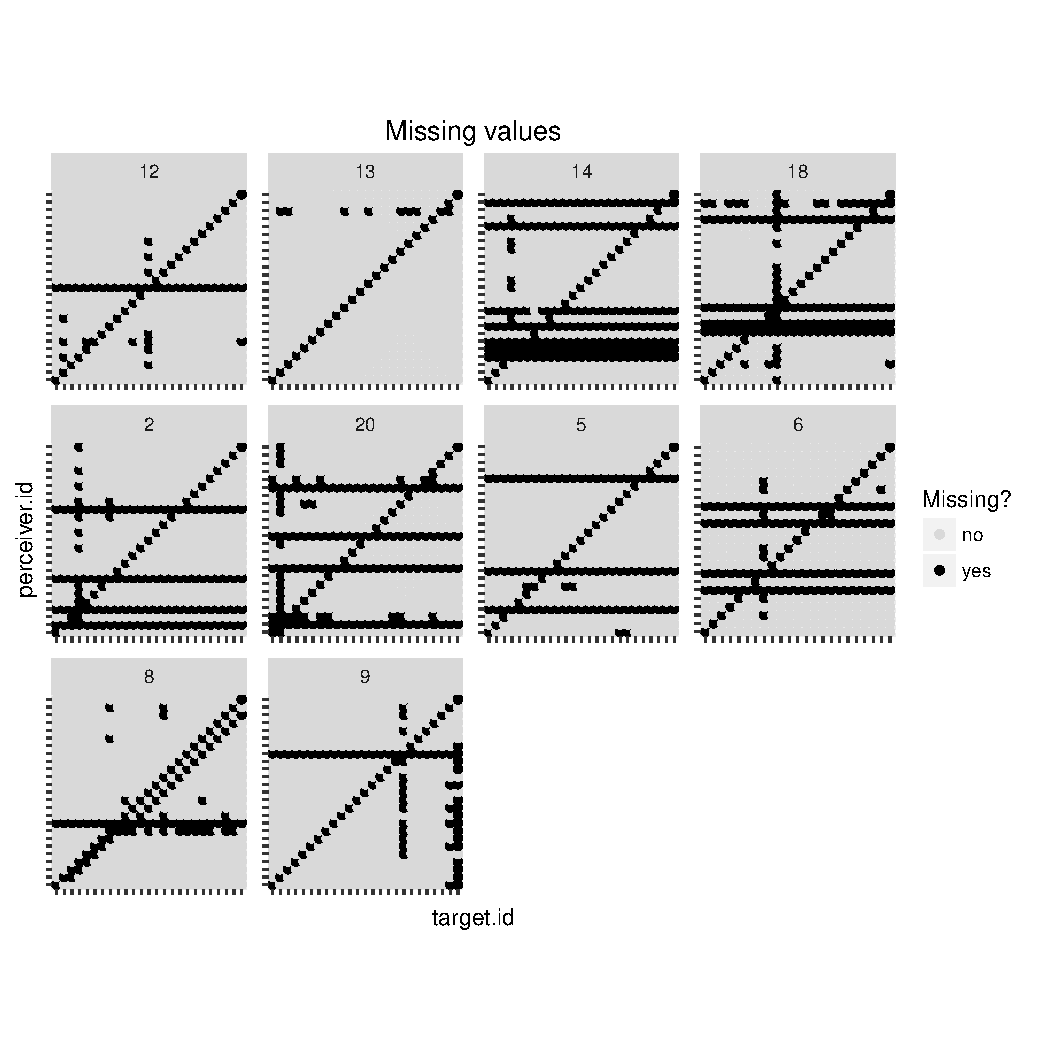
\includegraphics[width=\maxwidth]{Sweave-Files/Sw_unnamed-chunk-16-1} 
\end{knitrout}
\end{center}
\caption{Plot of missing values}
\label{fig:pmiss}
\end{figure}



If missing values are allowed by setting \texttt{na.rm=TRUE}, TripleR performs following three steps:
\begin{itemize}

	\item Participants which have too few data are removed both as perceivers and targets. Completely missing rows occur if participants do not rate anybody, for example because they were missing during data collection; missing columns might occur if participants cannot rate an unknown person. With a parameter (\texttt{minData}), this step can be adjusted to be more or less restrictive. \texttt{minData} defines the minimum of data points outside the diagonal which have to be present in each row or column. For example, one can define that at least two measurements (\texttt{minData=2}) should be present in each row or column.

	\item Missing values outside the diagonal are imputed as the average of the corresponding row and column mean1. Based on these imputed matrices, perceiver, target, and relationship effects are computed. Subsequently, relationship effects which were missing in the original data set are set as a missing value again.
	
	\item In the case of multiple variables (i.e., latent or bivariate analyses), participants are excluded listwise to ensure that all analyses are based on the same data set.
\end{itemize}


Based on extensive simulations we tentatively conclude that relatively small deviations from the true value can be expected if: 

\begin{itemize}
	\item For groups of 4 people <= 1 missing value
	\item For groups of 5 people <= 2 missing values
	\item For groups of 6 people <= 4 missing values
	\item For groups of 7 people <= 6 missing values
	\item For groups of 8 people <= 8 missing values
	\item For groups of 9 people <= 10 missing values
	\item Maximum 20\% missing values for groups with 10 or more people
\end{itemize}

More information on the handling of missing data and simulation studies can be found in \cite{Schonbrodt_Back_Schmukle_2012}.

As an example, we can analyze another built in data set with missing values:

\begin{knitrout}\small
\definecolor{shadecolor}{rgb}{0.969, 0.969, 0.969}\color{fgcolor}\begin{kframe}
\begin{alltt}
\hlkwd{data}\hlstd{(multiGroup)}

\hlcom{# by default, minData is set to 1 (i.e., at least one observation per row and column has}
\hlcom{# to be present)}
\hlstd{RR1miss} \hlkwb{<-} \hlkwd{RR}\hlstd{(ex} \hlopt{~} \hlstd{perceiver.id} \hlopt{*} \hlstd{target.id} \hlopt{|} \hlstd{group.id,} \hlkwc{data} \hlstd{= multiGroup,} \hlkwc{na.rm} \hlstd{=} \hlnum{TRUE}\hlstd{)}


\hlcom{# be more restrictive}
\hlstd{RR1miss} \hlkwb{<-} \hlkwd{RR}\hlstd{(ex} \hlopt{~} \hlstd{perceiver.id} \hlopt{*} \hlstd{target.id} \hlopt{|} \hlstd{group.id,} \hlkwc{data} \hlstd{= multiGroup,} \hlkwc{na.rm} \hlstd{=} \hlnum{TRUE}\hlstd{,} \hlkwc{minData} \hlstd{=} \hlnum{10}\hlstd{)}
\end{alltt}
\end{kframe}
\end{knitrout}



% subsection missing_values (end)



\subsection{Inspecting the results object} % (fold)
\label{sub:inspecting_the_results_object}
When a round robin analysis is performed (and stored in an object), not all information is displayed. When the object is printed (either by calling \texttt{print(object)}, e.g. \texttt{print(RR1)}, or by simple writing the name of the object into the R prompt, e.g. \texttt{RR1}), a custom \texttt{print} function is called, which displays the table of variance components, effects reliability estimates, and some other information. During the calculation, however, much more results are computed and stored in the object.

To see the structure of the object type \texttt{str(object)}:

\begin{knitrout}\small
\definecolor{shadecolor}{rgb}{0.969, 0.969, 0.969}\color{fgcolor}\begin{kframe}
\begin{alltt}
\hlkwd{str}\hlstd{(RR1)}
\end{alltt}
\begin{verbatim}
## List of 13
##  $ effects    :'data.frame':	54 obs. of  3 variables:
##   ..$ id        : chr [1:54] "1" "10" "11" "12" ...
##   ..$ liking_a.p: num [1:54] -0.477 -0.367 -0.406 0.152 0.663 ...
##   .. ..- attr(*, "type")= chr "actor"
##   .. ..- attr(*, "reliability")= num 0.937
##   ..$ liking_a.t: num [1:54] 0.26389 0.07728 0.00107 -0.40349 -0.33725 ...
##   .. ..- attr(*, "type")= chr "partner"
##   .. ..- attr(*, "reliability")= num 0.901
##  $ effectsRel :'data.frame':	2862 obs. of  4 variables:
##   ..$ actor.id    : Factor w/ 54 levels "1","2","3","4",..: 10 11 10 12 10 13 10 14 10 15 ...
##   ..$ partner.id  : Factor w/ 54 levels "1","2","3","4",..: 11 10 12 10 13 10 14 10 15 10 ...
##   ..$ dyad        : Factor w/ 1431 levels "1_01","1_02",..: 1 1 2 2 3 3 4 4 5 5 ...
##   ..$ relationship: num [1:2862] 1.186 1.149 0.591 0.591 -0.476 ...
##  $ effects.gm :'data.frame':	54 obs. of  3 variables:
##   ..$ id        : chr [1:54] "1" "10" "11" "12" ...
##   ..$ liking_a.p: num [1:54] 2.7 2.81 2.77 3.33 3.84 ...
##   .. ..- attr(*, "type")= chr "actor"
##   ..$ liking_a.t: num [1:54] 3.44 3.26 3.18 2.78 2.84 ...
##   .. ..- attr(*, "type")= chr "partner"
##  $ varComp    :'data.frame':	6 obs. of  7 variables:
##   ..$ type        : chr [1:6] "actor variance" "partner variance" "relationship variance" "error variance" ...
##   ..$ estimate    : num [1:6] 0.1717 0.1053 0.6088 NA 0.0141 ...
##   ..$ standardized: num [1:6] 0.194 0.119 0.687 NA 0.105 ...
##   ..$ se          : num [1:6] 0.0349 0.0223 0.0165 NA 0.02 ...
##   ..$ SEVAR       : num [1:6] 0.001221 0.000497 0.000273 NA 0.000401 ...
##   ..$ t.value     : num [1:6] 4.914 4.727 36.827 NA 0.703 ...
##   ..$ p.value     : num [1:6] 4.49e-06 8.62e-06 0.00 NA 4.85e-01 ...
##  $ relMat.av  : num [1:54, 1:54] NA 0.0715 0.1292 -0.4478 -0.7362 ...
##   ..- attr(*, "group.id")= chr "1"
##   ..- attr(*, "varname")= chr "liking_a"
##   ..- attr(*, "dimnames")=List of 2
##   .. ..$ : chr [1:54] "1" "10" "11" "12" ...
##   .. ..$ : chr [1:54] "1" "10" "11" "12" ...
##  $ relMat.diff: num [1:54, 1:54] NA -0.296 -0.333 -0.296 -0.741 ...
##   ..- attr(*, "group.id")= chr "1"
##   ..- attr(*, "varname")= chr "liking_a"
##   ..- attr(*, "dimnames")=List of 2
##   .. ..$ : chr [1:54] "1" "10" "11" "12" ...
##   .. ..$ : chr [1:54] "1" "10" "11" "12" ...
##  $ group.size : int 54
##  $ latent     : logi FALSE
##  $ anal.type  : chr "Univariate analysis of one round robin variable"
##  $ n.NA       : int 0
##  $ SEVAR      : Named num [1:6] 0.001221 0.000497 0.000273 NA 0.000401 ...
##   ..- attr(*, "names")= chr [1:6] "sesaa2" "sesbb2" "sescc2" "" ...
##  $ minVar     : num 0
##  $ se         : chr "LashleyBond"
##  - attr(*, "class")= chr "RRuni"
##  - attr(*, "group.size")= int 54
##  - attr(*, "varname")= chr "liking_a"
##  - attr(*, "self")= logi FALSE
\end{verbatim}
\end{kframe}
\end{knitrout}


Multiple data structures are stored in the object in list mode. Some objects are for internal use, others, however, are very important for subsequent analyses (see section \ref{sec:subsequent_analyses}).
You can access all stored objects via the \texttt{\$} operator. For example, the perceiver and target effects are stored in the \texttt{effects} object:

\begin{knitrout}\small
\definecolor{shadecolor}{rgb}{0.969, 0.969, 0.969}\color{fgcolor}\begin{kframe}
\begin{alltt}
\hlkwd{head}\hlstd{(RR1}\hlopt{$}\hlstd{effects)}
\end{alltt}
\begin{verbatim}
##    id liking_a.p   liking_a.t
## 1   1 -0.4768519  0.263888889
## 10 10 -0.3671652  0.077279202
## 11 11 -0.4063390  0.001068376
## 12 12  0.1520655 -0.403490028
## 13 13  0.6627493 -0.337250712
## 14 14  0.4141738  0.488247863
\end{verbatim}
\end{kframe}
\end{knitrout}

Following data objects might be relevant for subsequent analyses:
\begin{description}
	\item[effects] The perceiver and target effects. You access each effect by another \texttt{\$} operator; the effects have the same name like the original variable with a suffix for perceiver and target effect. Default suffixes are `.a' for actor and `.p' for partner effect (if \texttt{RR.style} is set to \texttt{behavior}), or `.p' for perceiver and `.t' for target effect (if \texttt{RR.style} is set to \texttt{perception}). For example, if your original variable is called \texttt{liking}, you can access the perceiver effect by \texttt{RR1\$effects\$liking.p}. If self ratings are present in the data set, they are also returned with the default suffix \texttt{.s}. You can inspect the effects by typing \texttt{str(RR1\$effects)}.
	In latent analyses, effects are returned as the average of the two underlying manifest effects.
	\item[effects.gm] Actor and partner effects with group mean added.
	\item[effectsRel] A data frame in long format which corresponds to the \texttt{n x n} matrix of relationship effects
	\item[varComp] A data frame with the absolute and standardized variance components and their respective significance tests (this object is printed int the \texttt{print} function of an \texttt{RR} object).
	\item[group.var] In the multi group case: display the group variance.
\end{description}

In section \ref{sec:subsequent_analyses} (Subsequent Analyses) it is explained how follow up analyses using the perceiver and target effects, and the variance components can be done.
% subsection inspecting_the_results_object (end)






\section{Plots} % (fold)
\label{sec:plots}

Several plots can be made from the result objects. Simply type \texttt{plot(RR\_object)} to see the standard variance plot associated with each analysis. The main difference between plots is whether you have multiple groups or a single round robin group.

\begin{knitrout}\small
\definecolor{shadecolor}{rgb}{0.969, 0.969, 0.969}\color{fgcolor}\begin{kframe}
\begin{alltt}
\hlcom{# see Figure 1}
\hlkwd{plot}\hlstd{(RR1)}
\end{alltt}
\end{kframe}
\end{knitrout}

\begin{figure} 
\begin{center} 
\begin{knitrout}\small
\definecolor{shadecolor}{rgb}{0.969, 0.969, 0.969}\color{fgcolor}
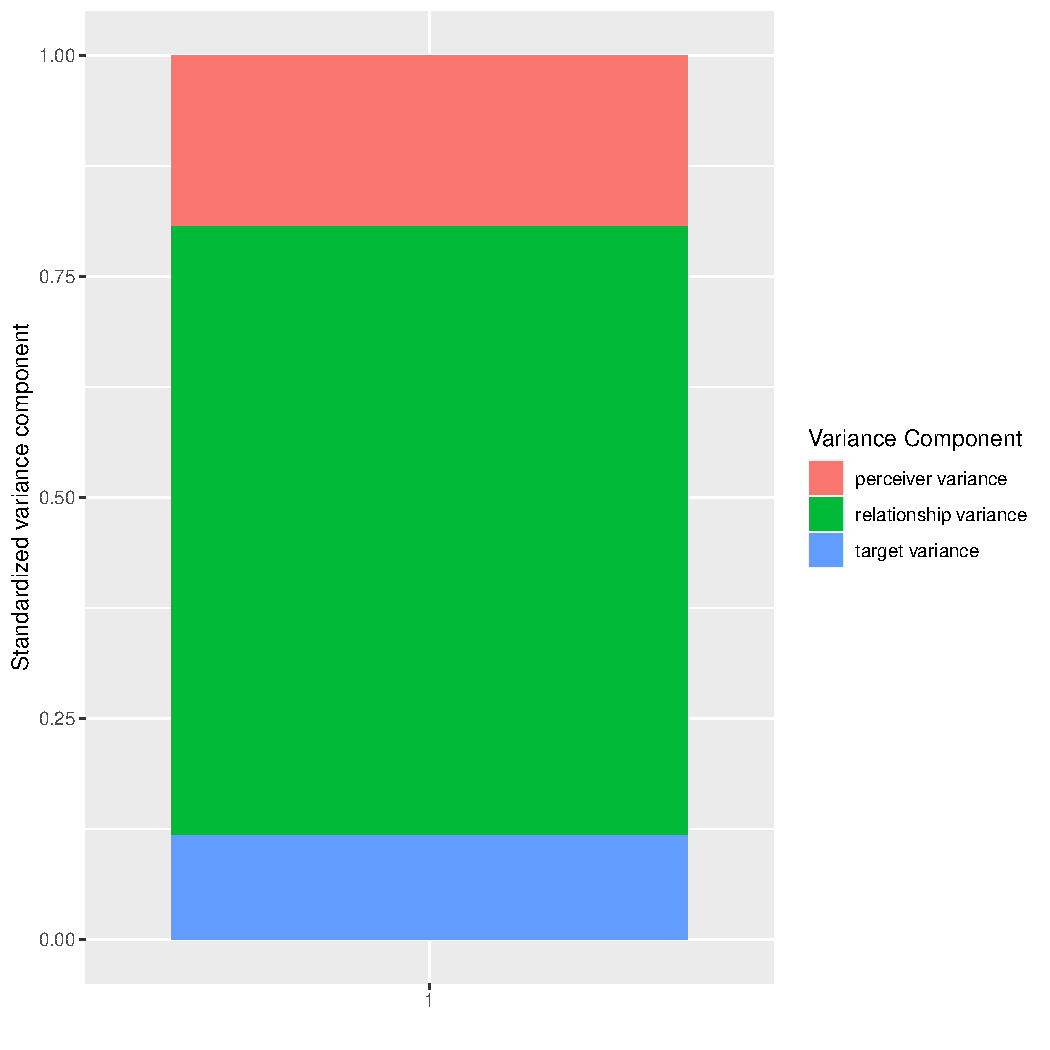
\includegraphics[width=\maxwidth]{Sweave-Files/Sw_unnamed-chunk-21-1} 
\end{knitrout}
\end{center}
\caption{Variance decomposition of a single round robin group}
\label{fig:one}
\end{figure}




\begin{knitrout}\small
\definecolor{shadecolor}{rgb}{0.969, 0.969, 0.969}\color{fgcolor}\begin{kframe}
\begin{alltt}
\hlcom{# see Figure 2}
\hlkwd{plot}\hlstd{(RR1m)}
\end{alltt}
\end{kframe}
\end{knitrout}

\begin{figure} 
\begin{center} 
\begin{knitrout}\small
\definecolor{shadecolor}{rgb}{0.969, 0.969, 0.969}\color{fgcolor}\begin{kframe}


{\ttfamily\noindent\color{warningcolor}{\#\# Warning: Removed 1 rows containing missing values (geom\_segment).}}\end{kframe}
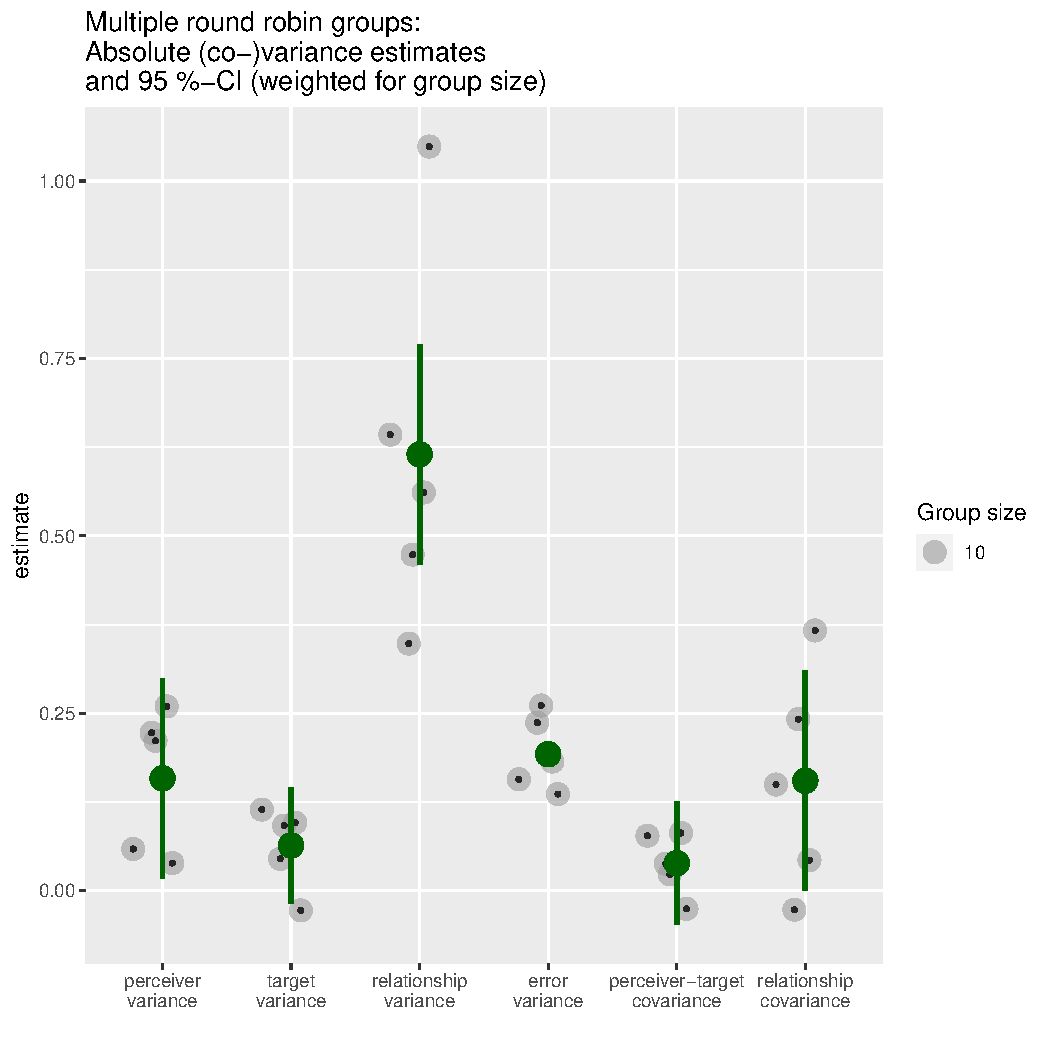
\includegraphics[width=\maxwidth]{Sweave-Files/Sw_unnamed-chunk-23-1} 
\end{knitrout}
\end{center}
\caption{Variance decomposition of multiple round robin groups, latent analysis}
\label{fig:two}
\end{figure}


You can also try different parameters:
\begin{description}
	\item[measure] =\texttt{behavior} (default) or \texttt{perception}: changes the labels of the plots
	\item[geom (single groups)] = \texttt{bar} (default) or \texttt{pie}: show variance components as stacked bars or as a pie chart
	\item[geom (multiple groups)] = \texttt{scatter} (default) or \texttt{bar}: show variance components of all groups as scatter plots with confidence intervals or as a bar charts
	\item[connect (multiple groups)] = \texttt{FALSE} (default) or \texttt{TRUE}: connect the dots of each group in the scatter plot (usually this looks very cluttered and should not be turned on)
	\item[conf.level (multiple groups)] (defaults to 0.95) defines the size of the confidence interval in the scatter plot
\end{description}


Hence you can try several combinations of these parameters, e.g.:

\begin{knitrout}\small
\definecolor{shadecolor}{rgb}{0.969, 0.969, 0.969}\color{fgcolor}\begin{kframe}
\begin{alltt}
\hlkwd{plot}\hlstd{(RR1,} \hlkwc{measure} \hlstd{=} \hlstr{"perception"}\hlstd{,} \hlkwc{geom} \hlstd{=} \hlstr{"pie"}\hlstd{)}
\end{alltt}
\end{kframe}
\end{knitrout}



\begin{knitrout}\small
\definecolor{shadecolor}{rgb}{0.969, 0.969, 0.969}\color{fgcolor}\begin{kframe}
\begin{alltt}
\hlkwd{plot}\hlstd{(RR1,} \hlkwc{measure} \hlstd{=} \hlstr{"behavior"}\hlstd{,} \hlkwc{geom} \hlstd{=} \hlstr{"pie"}\hlstd{)}
\end{alltt}
\end{kframe}
\end{knitrout}



\begin{knitrout}\small
\definecolor{shadecolor}{rgb}{0.969, 0.969, 0.969}\color{fgcolor}\begin{kframe}
\begin{alltt}
\hlkwd{plot}\hlstd{(RR1m,} \hlkwc{measure} \hlstd{=} \hlstr{"perception"}\hlstd{,} \hlkwc{geom} \hlstd{=} \hlstr{"bar"}\hlstd{)}
\end{alltt}
\end{kframe}
\end{knitrout}


\begin{knitrout}\small
\definecolor{shadecolor}{rgb}{0.969, 0.969, 0.969}\color{fgcolor}\begin{kframe}
\begin{alltt}
\hlkwd{plot}\hlstd{(RR1m,} \hlkwc{conf.level} \hlstd{=} \hlnum{0.5}\hlstd{,} \hlkwc{connect} \hlstd{=} \hlnum{TRUE}\hlstd{)}
\end{alltt}
\end{kframe}
\end{knitrout}




The plot function returns a \texttt{ggplot2} object, which in turn can be altered (e.g., you can change the title, the axes labels, the colors, etc.). For more information, please consult the \texttt{ggplot2} documentation.


% section plots (end)






\section{Formatting the output} 
As mentioned above, two nomenclatures have been established, depending on whether behaviors or interpersonal perceptions are assessed. While internally always the labels \emph{actor} and \emph{partner} are used, the summary output can be customized by specifying whether the measure is a \texttt{behavior} or a \texttt{perception} (default is \emph{behavior}). In bivariate analyses, both variables can be specified, e.g. \texttt{measure1=`behavior', measure2=`perception'}, or all other combinations.

Possible combinations are for the univariate case: \texttt{measure=c(`behavior', `perception')}; and for the bivariate case: \texttt{measure1 = c(`behavior', `perception')}, \texttt{measure2 = c(`behavior', `perception')}, and the special case \texttt{measure1=`perception', measure2=`metaperception'} (in the latter, special labels are used for bivariate covariances, see output below).

\begin{knitrout}\small
\definecolor{shadecolor}{rgb}{0.969, 0.969, 0.969}\color{fgcolor}\begin{kframe}
\begin{alltt}
\hlkwd{print}\hlstd{(RR1,} \hlkwc{measure1} \hlstd{=} \hlstr{"perception"}\hlstd{)}
\end{alltt}
\begin{verbatim}
## Round-Robin object ('RR'), calculated by TripleR
## ------------------------------------------------
## Univariate analysis of one round robin variable
## 
## Univariate analyses for: liking_a 
## ---------
## Round robin analysis for a single group; using the formula of Lashley & Bond (1997).
## 
##                             estimate standardized    se t.value p.value
## perceiver variance             0.172        0.194 0.035   4.914   0.000
## target variance                0.105        0.119 0.022   4.727   0.000
## relationship variance          0.609        0.687 0.017  36.827   0.000
## error variance                    NA           NA    NA      NA      NA
## perceiver-target covariance    0.014        0.105 0.020   0.703   0.485
## relationship covariance        0.080        0.131 0.017   4.809   0.000
## Perceiver effect reliability: .937 
## Target effect reliability: .901 
## NULL
\end{verbatim}
\end{kframe}
\end{knitrout}

\par\vspace{5mm}

\begin{knitrout}\small
\definecolor{shadecolor}{rgb}{0.969, 0.969, 0.969}\color{fgcolor}\begin{kframe}
\begin{alltt}
\hlkwd{print}\hlstd{(RR4,} \hlkwc{measure1} \hlstd{=} \hlstr{"behavior"}\hlstd{,} \hlkwc{measure2} \hlstd{=} \hlstr{"perception"}\hlstd{)}
\end{alltt}
\begin{verbatim}
## $univariate
## $univariate[[1]]
## Round-Robin object ('RR'), calculated by TripleR
## ------------------------------------------------
## Latent construct analysis of one construct measured by two round robin variables
## 
## Univariate analyses for: liking_a/liking_b 
## ---------
## Round robin analysis for a single group; using the formula of Lashley & Bond (1997).
## 
##                          estimate standardized    se t.value p.value
## actor variance              0.161        0.164 0.036   4.524   0.000
## partner variance            0.105        0.107 0.023   4.678   0.000
## relationship variance       0.507        0.518 0.016  31.125   0.000
## error variance              0.206        0.211    NA      NA      NA
## actor-partner covariance    0.012        0.094 0.021   0.573   0.569
## relationship covariance     0.079        0.156 0.016   4.861   0.000
## Actor effect reliability: .865 
## Partner effect reliability: .893 
## Relationship effect reliability: .852 
## NULL
## 
## $univariate[[2]]
## Round-Robin object ('RR'), calculated by TripleR
## ------------------------------------------------
## Latent construct analysis of one construct measured by two round robin variables
## 
## Univariate analyses for: metaliking_a/metaliking_b 
## ---------
## Round robin analysis for a single group; using the formula of Lashley & Bond (1997).
## 
##                          estimate standardized    se t.value p.value
## actor variance              0.148        0.217 0.031   4.729   0.000
## partner variance            0.026        0.038 0.007   3.978   0.000
## relationship variance       0.357        0.522 0.012  30.568   0.000
## error variance              0.153        0.223    NA      NA      NA
## actor-partner covariance    0.000        0.002 0.011   0.014   0.989
## relationship covariance     0.071        0.197 0.012   6.034   0.000
## Actor effect reliability: .899 
## Partner effect reliability: .761 
## Relationship effect reliability: .841 
## NULL
## 
## 
## $bivariate
##                                         type    estimate standardized         se
## sesaf                 actor-actor covariance 0.091737622   0.59330340 0.02722553
## sesbg             partner-partner covariance 0.048567501   0.92809821 0.01133202
## sesag               actor-partner covariance 0.007382948   0.11407774 0.01093178
## sesbf               partner-actor covariance 0.003979599   0.03183066 0.01901930
## sesch  intrapersonal relationship covariance 0.329513319   0.77420495 0.01162831
## seschs interpersonal relationship covariance 0.075332206   0.17699608 0.01162831
##             biSEVAR    t.value      p.value
## sesaf  0.0007412297  3.3695434 1.410120e-03
## sesbg  0.0001284146  4.2858651 7.715979e-05
## sesag  0.0001195038  0.6753656 5.023795e-01
## sesbf  0.0003617339  0.2092400 8.350631e-01
## sesch  0.0001352176 28.3371645 0.000000e+00
## seschs 0.0001352176  6.4783454 3.111736e-08
## 
## $anal.type
## [1] "Bivariate analysis of two constructs, each measured by two round robin variables"
## 
## $minVar
## [1] 0
## 
## $se
## [1] "LashleyBond"
## 
## attr(,"class")
## [1] "RR"
## attr(,"group.size")
## [1] 54
\end{verbatim}
\end{kframe}
\end{knitrout}
\par\vspace{5mm}
\begin{knitrout}\small
\definecolor{shadecolor}{rgb}{0.969, 0.969, 0.969}\color{fgcolor}\begin{kframe}
\begin{alltt}
\hlkwd{print}\hlstd{(RR4,} \hlkwc{measure1} \hlstd{=} \hlstr{"perception"}\hlstd{,} \hlkwc{measure2} \hlstd{=} \hlstr{"metaperception"}\hlstd{)}
\end{alltt}
\begin{verbatim}
## $univariate
## $univariate[[1]]
## Round-Robin object ('RR'), calculated by TripleR
## ------------------------------------------------
## Latent construct analysis of one construct measured by two round robin variables
## 
## Univariate analyses for: liking_a/liking_b 
## ---------
## Round robin analysis for a single group; using the formula of Lashley & Bond (1997).
## 
##                             estimate standardized    se t.value p.value
## perceiver variance             0.161        0.164 0.036   4.524   0.000
## target variance                0.105        0.107 0.023   4.678   0.000
## relationship variance          0.507        0.518 0.016  31.125   0.000
## error variance                 0.206        0.211    NA      NA      NA
## perceiver-target covariance    0.012        0.094 0.021   0.573   0.569
## relationship covariance        0.079        0.156 0.016   4.861   0.000
## Perceiver effect reliability: .865 
## Target effect reliability: .893 
## Relationship effect reliability: .852 
## NULL
## 
## $univariate[[2]]
## Round-Robin object ('RR'), calculated by TripleR
## ------------------------------------------------
## Latent construct analysis of one construct measured by two round robin variables
## 
## Univariate analyses for: metaliking_a/metaliking_b 
## ---------
## Round robin analysis for a single group; using the formula of Lashley & Bond (1997).
## 
##                             estimate standardized    se t.value p.value
## perceiver variance             0.148        0.217 0.031   4.729   0.000
## target variance                0.026        0.038 0.007   3.978   0.000
## relationship variance          0.357        0.522 0.012  30.568   0.000
## error variance                 0.153        0.223    NA      NA      NA
## perceiver-target covariance    0.000        0.002 0.011   0.014   0.989
## relationship covariance        0.071        0.197 0.012   6.034   0.000
## Perceiver effect reliability: .899 
## Target effect reliability: .761 
## Relationship effect reliability: .841 
## NULL
## 
## 
## $bivariate
##                                         type    estimate standardized         se
## sesaf                 actor-actor covariance 0.091737622   0.59330340 0.02722553
## sesbg             partner-partner covariance 0.048567501   0.92809821 0.01133202
## sesag               actor-partner covariance 0.007382948   0.11407774 0.01093178
## sesbf               partner-actor covariance 0.003979599   0.03183066 0.01901930
## sesch  intrapersonal relationship covariance 0.329513319   0.77420495 0.01162831
## seschs interpersonal relationship covariance 0.075332206   0.17699608 0.01162831
##             biSEVAR    t.value      p.value
## sesaf  0.0007412297  3.3695434 1.410120e-03
## sesbg  0.0001284146  4.2858651 7.715979e-05
## sesag  0.0001195038  0.6753656 5.023795e-01
## sesbf  0.0003617339  0.2092400 8.350631e-01
## sesch  0.0001352176 28.3371645 0.000000e+00
## seschs 0.0001352176  6.4783454 3.111736e-08
## 
## $anal.type
## [1] "Bivariate analysis of two constructs, each measured by two round robin variables"
## 
## $minVar
## [1] 0
## 
## $se
## [1] "LashleyBond"
## 
## attr(,"class")
## [1] "RR"
## attr(,"group.size")
## [1] 54
\end{verbatim}
\end{kframe}
\end{knitrout}
\par\vspace{5mm}

As you can see, typical labels from different research traditions, like `generalized reciprocity metaperception' or `perceiver meta-accuracy' are automatically printed to ease interpretation of the results.

A convenient short cut to achieve this styling is the function \texttt{RR.style}. You can call this function once at the beginning of your script, and all subsequent analyses will be labelled accordingly. For details see \texttt{?RR.style}.



\section{Subsequent analyses} % (fold)
\label{sec:subsequent_analyses}
Usually one does not only want to know about the variance components and the within-SRM correlations. Often, we want to correlate the perceiver and target effects with the self-ratings, with external personality questionnaires, or demographic variables. To do this, we can extract the perceiver/ target effects from the RR-object, combine them with the other data (e.g., questionnaire scales) in another data frame, and do which ever analysis we like.

\emph{Be careful:} in RR objects one cannot be sure about the order and the completeness of the effects. That means, perceivers can be reordered and their order might be different from that in the original data set. Furthermore, if some participants are only perceivers or only targets they are removed prior to to the social relations analyses, and do not appear in the actor/ partner effects. Hence, merging of RR effects and other data \emph{always} has to be done using the \texttt{merge} command. As non-round robin variables usually are assigned to the perceiver ID, consequently merging should be done along the perceiver ID).

The data set \texttt{multiGroup} contains round robin ratings and self ratings of extraversion, which will serve as an extended example:

\begin{knitrout}\small
\definecolor{shadecolor}{rgb}{0.969, 0.969, 0.969}\color{fgcolor}\begin{kframe}
\begin{alltt}
\hlcom{# calculate the SRM}
\hlkwd{data}\hlstd{(multiGroup)}
\hlkwd{RR.style}\hlstd{(}\hlstr{"perception"}\hlstd{)}
\hlstd{RR1m} \hlkwb{<-} \hlkwd{RR}\hlstd{(ex} \hlopt{~} \hlstd{perceiver.id} \hlopt{*} \hlstd{target.id} \hlopt{|} \hlstd{group.id,} \hlkwc{data} \hlstd{= multiGroup,} \hlkwc{na.rm} \hlstd{=} \hlnum{TRUE}\hlstd{)}
\end{alltt}


{\ttfamily\noindent\color{warningcolor}{\#\# Warning: ex : \ 4 \ participant(s) have been excluded from group 2 due to exceedingly missing data; id(s) = 90202, 90204, 90208, 90217 .}}

{\ttfamily\noindent\color{warningcolor}{\#\# Warning: ex : \ 3 \ participant(s) have been excluded from group 5 due to exceedingly missing data; id(s) = 90509, 90504, 90521 .}}

{\ttfamily\noindent\color{warningcolor}{\#\# Warning: ex : \ 4 \ participant(s) have been excluded from group 6 due to exceedingly missing data; id(s) = 90606, 90608, 90614, 90616 .}}

{\ttfamily\noindent\color{warningcolor}{\#\# Warning: ex : \ 1 \ participant(s) have been excluded from group 8 due to exceedingly missing data; id(s) = 90811 .}}

{\ttfamily\noindent\color{warningcolor}{\#\# Warning: ex : \ 1 \ participant(s) have been excluded from group 9 due to exceedingly missing data; id(s) = 90918 .}}

{\ttfamily\noindent\color{warningcolor}{\#\# Warning: ex : \ 1 \ participant(s) have been excluded from group 12 due to exceedingly missing data; id(s) = 91213 .}}

{\ttfamily\noindent\color{warningcolor}{\#\# Warning: ex : \ 6 \ participant(s) have been excluded from group 14 due to exceedingly missing data; id(s) = 91404, 91405, 91406, 91408, 91424, 91421 .}}

{\ttfamily\noindent\color{warningcolor}{\#\# Warning: ex : \ 4 \ participant(s) have been excluded from group 18 due to exceedingly missing data; id(s) = 91807, 91808, 91810, 91821 .}}

{\ttfamily\noindent\color{warningcolor}{\#\# Warning: ex : \ 4 \ participant(s) have been excluded from group 20 due to exceedingly missing data; id(s) = 92002, 92009, 92013, 92019 .}}\begin{alltt}
\hlcom{# extract the effects}
\hlstd{eff} \hlkwb{<-} \hlstd{RR1m}\hlopt{$}\hlstd{effects}
\hlkwd{head}\hlstd{(eff)}
\end{alltt}
\begin{verbatim}
##      id group.id        ex.p       ex.t       ex.s
## 1 90201        2 -0.59649123  0.6892231  1.1428571
## 2 90203        2  0.73934837 -0.5939850  1.1428571
## 3 90205        2  0.04511278  0.5213033  0.1428571
## 4 90206        2 -0.49373434  0.7443609  0.1428571
## 5 90207        2  0.03007519 -1.7794486 -1.8571429
## 6 90209        2 -0.16541353  2.3107769  2.1428571
\end{verbatim}
\end{kframe}
\end{knitrout}


As perceiver and target effects are corrected for group membership in \emph{g} groups, according to Kenny et al. (2006) partial correlations should be used when these effects are correlated with external (non-SRM) variables (i.e. external variables like self ratings also have to be controlled for group membership). `Controlling for group membership' by \emph{g}-1 dummy variables is equivalent to group centering all measures. As the self ratings returned by \texttt{RR\$effects} already are centered on group level, all variables (perceiver \& target effects, self ratings) already are controlled for group membership. 


Correlations between group centered variables and partial correlations between their non-centered counterparts \emph{controlled for group membership} are exactly the same. However, when controlling for group membership, one loses \emph{g}-1 degrees of freedom, hence their test of significance is more conservative.

For the calculation of these partial correlations, you can either export the calculated effects to another software which can calculate partial correlations (for export, see section \ref{sec:export}), or you can calculate these partial correlations in R.

\subsection{Assumed similarity and self-other agreement: Correlations with self-ratings} % (fold)

In data sets where self ratings are provided (in the diagonal of the round-robin matrix), the output prints correlations between self ratings and perceiver and target effects (also see function \texttt{selfCor}). In the case of multiple groups, these correlations are controlled for group membership, but are not disattenuated for perceiver/target effect unreliability (for an example on how to disattenuate these correlations, see below). In the following you find an example of such an analysis for the multiGroup data set:

\begin{knitrout}\small
\definecolor{shadecolor}{rgb}{0.969, 0.969, 0.969}\color{fgcolor}\begin{kframe}
\begin{alltt}
\hlkwd{data}\hlstd{(multiGroup)}

\hlkwd{RR.style}\hlstd{(}\hlstr{"p"}\hlstd{)}
\hlcom{# a single group}
\hlstd{RR1} \hlkwb{<-} \hlkwd{RR}\hlstd{(ex} \hlopt{~} \hlstd{perceiver.id} \hlopt{*} \hlstd{target.id} \hlopt{|} \hlstd{group.id,} \hlkwc{data} \hlstd{= multiGroup[multiGroup}\hlopt{$}\hlstd{group.id} \hlopt{==}
    \hlstr{"2"}\hlstd{, ],} \hlkwc{na.rm} \hlstd{=} \hlnum{TRUE}\hlstd{)}
\end{alltt}


{\ttfamily\noindent\color{warningcolor}{\#\# Warning: ex : \ 4 \ participant(s) have been excluded from group 2 due to exceedingly missing data; id(s) = 90202, 90204, 90208, 90217 .}}\begin{alltt}
\hlkwd{selfCor}\hlstd{(RR1)}
\end{alltt}
\begin{verbatim}
## NULL
## 
## 
## Correlations with self ratings:
##                                                        r    t     df     p   
## self rating with Perceiver effect (assumed similarity) .393 1.862 19.000 .078
## self rating with Target effect (self-other agreement)  .527 2.705 19.000 .014
\end{verbatim}
\begin{alltt}
\hlcom{# multiple groups}
\hlstd{RR2} \hlkwb{<-} \hlkwd{RR}\hlstd{(ex} \hlopt{~} \hlstd{perceiver.id} \hlopt{*} \hlstd{target.id} \hlopt{|} \hlstd{group.id,} \hlkwc{data} \hlstd{= multiGroup,} \hlkwc{na.rm} \hlstd{=} \hlnum{TRUE}\hlstd{)}
\end{alltt}


{\ttfamily\noindent\color{warningcolor}{\#\# Warning: ex : \ 4 \ participant(s) have been excluded from group 2 due to exceedingly missing data; id(s) = 90202, 90204, 90208, 90217 .}}

{\ttfamily\noindent\color{warningcolor}{\#\# Warning: ex : \ 3 \ participant(s) have been excluded from group 5 due to exceedingly missing data; id(s) = 90509, 90504, 90521 .}}

{\ttfamily\noindent\color{warningcolor}{\#\# Warning: ex : \ 4 \ participant(s) have been excluded from group 6 due to exceedingly missing data; id(s) = 90606, 90608, 90614, 90616 .}}

{\ttfamily\noindent\color{warningcolor}{\#\# Warning: ex : \ 1 \ participant(s) have been excluded from group 8 due to exceedingly missing data; id(s) = 90811 .}}

{\ttfamily\noindent\color{warningcolor}{\#\# Warning: ex : \ 1 \ participant(s) have been excluded from group 9 due to exceedingly missing data; id(s) = 90918 .}}

{\ttfamily\noindent\color{warningcolor}{\#\# Warning: ex : \ 1 \ participant(s) have been excluded from group 12 due to exceedingly missing data; id(s) = 91213 .}}

{\ttfamily\noindent\color{warningcolor}{\#\# Warning: ex : \ 6 \ participant(s) have been excluded from group 14 due to exceedingly missing data; id(s) = 91404, 91405, 91406, 91408, 91424, 91421 .}}

{\ttfamily\noindent\color{warningcolor}{\#\# Warning: ex : \ 4 \ participant(s) have been excluded from group 18 due to exceedingly missing data; id(s) = 91807, 91808, 91810, 91821 .}}

{\ttfamily\noindent\color{warningcolor}{\#\# Warning: ex : \ 4 \ participant(s) have been excluded from group 20 due to exceedingly missing data; id(s) = 92002, 92009, 92013, 92019 .}}\begin{alltt}
\hlstd{c1} \hlkwb{<-} \hlkwd{selfCor}\hlstd{(RR2)}
\end{alltt}
\begin{verbatim}
## NULL
## 
## 
## Partial correlations with self ratings (controlled for group membership):
##                                                        r    t      df      p   
## self rating with Perceiver effect (assumed similarity) .307 4.634  206.000 .000
## self rating with Target effect (self-other agreement)  .609 11.012 206.000 .000
\end{verbatim}
\end{kframe}
\end{knitrout}


In this analysis, we find a considerable self-other agreement of extraversion ratings $r_{ex.target,ex.self}=0.609$.

Correlations which are calculated by SOREMO.exe are by default disattenuated for perceiver and/or target effect unreliability. To replicate these results, you have to disattenuate the obtained correlations by following formula:

$r_{disatt} = r_{raw}*\frac{1}{\sqrt{Rel_{target effect}}}$

Hence, the disattenuated correlation $r_{ex.target,ex.self}$ would be $0.609*\frac{1}{\sqrt{0.935}} = 0.629$.






\subsection{Calculating partial correlations with external variables: Treating groups as fixed effects} % (fold)
\label{subsec:part}

Probably, you have other external variables except the self rating. These are variables which are not assessed with the round robin design, but rather individual variables like self ratings of personality, or demographic variables. The variable \texttt{narc} (= narcissism) in the data set \texttt{multiNarc} is such a variable: it is a self rating of narcissism. The function \texttt{parCor} now helps to calculate the partial correlation between an SRM effect and this external variable, controlled for group membership:

\begin{knitrout}\small
\definecolor{shadecolor}{rgb}{0.969, 0.969, 0.969}\color{fgcolor}\begin{kframe}
\begin{alltt}
\hlkwd{data}\hlstd{(multiGroup)}
\hlkwd{data}\hlstd{(multiNarc)}

\hlcom{# show the first lines of multiNarc:}
\hlkwd{head}\hlstd{(multiNarc)}
\end{alltt}
\begin{verbatim}
##          id narc
## 90201 90201    7
## 90205 90205    6
## 90207 90207    3
## 90209 90209   12
## 90210 90210    8
## 90212 90212    6
\end{verbatim}
\begin{alltt}
\hlkwd{RR.style}\hlstd{(}\hlstr{"p"}\hlstd{)}
\hlcom{# calculate SRA effects for extraversion ratings}
\hlstd{RR1} \hlkwb{<-} \hlkwd{RR}\hlstd{(ex} \hlopt{~} \hlstd{perceiver.id} \hlopt{*} \hlstd{target.id} \hlopt{|} \hlstd{group.id, multiGroup,} \hlkwc{na.rm} \hlstd{=} \hlnum{TRUE}\hlstd{)}
\end{alltt}


{\ttfamily\noindent\color{warningcolor}{\#\# Warning: ex : \ 4 \ participant(s) have been excluded from group 2 due to exceedingly missing data; id(s) = 90202, 90204, 90208, 90217 .}}

{\ttfamily\noindent\color{warningcolor}{\#\# Warning: ex : \ 3 \ participant(s) have been excluded from group 5 due to exceedingly missing data; id(s) = 90509, 90504, 90521 .}}

{\ttfamily\noindent\color{warningcolor}{\#\# Warning: ex : \ 4 \ participant(s) have been excluded from group 6 due to exceedingly missing data; id(s) = 90606, 90608, 90614, 90616 .}}

{\ttfamily\noindent\color{warningcolor}{\#\# Warning: ex : \ 1 \ participant(s) have been excluded from group 8 due to exceedingly missing data; id(s) = 90811 .}}

{\ttfamily\noindent\color{warningcolor}{\#\# Warning: ex : \ 1 \ participant(s) have been excluded from group 9 due to exceedingly missing data; id(s) = 90918 .}}

{\ttfamily\noindent\color{warningcolor}{\#\# Warning: ex : \ 1 \ participant(s) have been excluded from group 12 due to exceedingly missing data; id(s) = 91213 .}}

{\ttfamily\noindent\color{warningcolor}{\#\# Warning: ex : \ 6 \ participant(s) have been excluded from group 14 due to exceedingly missing data; id(s) = 91404, 91405, 91406, 91408, 91424, 91421 .}}

{\ttfamily\noindent\color{warningcolor}{\#\# Warning: ex : \ 4 \ participant(s) have been excluded from group 18 due to exceedingly missing data; id(s) = 91807, 91808, 91810, 91821 .}}

{\ttfamily\noindent\color{warningcolor}{\#\# Warning: ex : \ 4 \ participant(s) have been excluded from group 20 due to exceedingly missing data; id(s) = 92002, 92009, 92013, 92019 .}}\begin{alltt}
\hlcom{# merge variables}
\hlstd{dat} \hlkwb{<-} \hlkwd{merge}\hlstd{(RR1}\hlopt{$}\hlstd{effects, multiNarc,} \hlkwc{by} \hlstd{=} \hlstr{"id"}\hlstd{)}

\hlcom{# parCor(x, y, z): partial correlation between x and y, controlled for group memberhsip z}
\hlkwd{parCor}\hlstd{(dat}\hlopt{$}\hlstd{ex.t, dat}\hlopt{$}\hlstd{narc, dat}\hlopt{$}\hlstd{group.id)}
\end{alltt}
\begin{verbatim}
## $par.cor
## [1] 0.7620022
## 
## $t.value
## [1] 15.91813
## 
## $df
## [1] 183
## 
## $p
## [1] 0
\end{verbatim}
\end{kframe}
\end{knitrout}



\subsection{Calculating partial correlations with external variables: Treating groups as random effects - the multilevel approach} % (fold)
\label{subsec:ml}


Using the approach of group centering, groups are treated as fixed factors. Both conceptually and by means of computations it might be preferable to treat groups as random factors (which, however, requires a sufficient number of groups). When using a multilevel approach, we would like to keep the group variance in our dependent variable (as the multilevel modeling takes care of this), hence we use the effects with group mean added (\texttt{effects.gm}) and the raw self ratings. Using a multilevel modeling approach, the calculation would look like the following:

\begin{knitrout}\small
\definecolor{shadecolor}{rgb}{0.969, 0.969, 0.969}\color{fgcolor}\begin{kframe}
\begin{alltt}
\hlkwd{library}\hlstd{(lme4)}
\end{alltt}


{\ttfamily\noindent\itshape\color{messagecolor}{\#\# Lade n"{}otiges Paket: Matrix}}\begin{alltt}
\hlstd{eff.gm} \hlkwb{<-} \hlstd{RR1m}\hlopt{$}\hlstd{effects.gm}
\hlcom{# scale all continuous variables to obtain standardized estimates}
\hlstd{eff.gm[,} \hlnum{3}\hlopt{:}\hlnum{5}\hlstd{]} \hlkwb{<-} \hlkwd{apply}\hlstd{(eff.gm[,} \hlnum{3}\hlopt{:}\hlnum{5}\hlstd{],} \hlnum{2}\hlstd{, scale)}

\hlcom{# Allow the intercept to vary between groups (this is equivalent to the fixed effects}
\hlcom{# approach, only with random effects).  Additionally, allow slopes to vary:}
\hlkwd{lmer}\hlstd{(ex.s} \hlopt{~} \hlstd{ex.t} \hlopt{+} \hlstd{(ex.t} \hlopt{|} \hlstd{group.id), eff.gm)}
\end{alltt}


{\ttfamily\noindent\itshape\color{messagecolor}{\#\# boundary (singular) fit: see help('isSingular')}}\begin{verbatim}
## Linear mixed model fit by REML ['lmerMod']
## Formula: ex.s ~ ex.t + (ex.t | group.id)
##    Data: eff.gm
## REML criterion at convergence: 525.5937
## Random effects:
##  Groups   Name        Std.Dev.  Corr
##  group.id (Intercept) 0.000e+00     
##           ex.t        1.860e-08  NaN
##  Residual             8.012e-01     
## Number of obs: 217, groups:  group.id, 10
## Fixed Effects:
## (Intercept)         ex.t  
##   1.162e-15    6.009e-01  
## optimizer (nloptwrap) convergence code: 0 (OK) ; 0 optimizer warnings; 1 lme4 warnings
\end{verbatim}
\end{kframe}
\end{knitrout}


The multilevel analysis reveals a self-other agreement of extraversion ratings $\beta_{ex.target,ex.self}=.601$. As there is no random variance of the group level in this analysis (and also no random variance of the slopes), the result is virtually the same as in the fixed effects analysis.

For principal reasons, the \texttt{lme4} package does not report p values, as it is not clear how to compute the degrees of freedoms in multilevel models\footnote{https://stat.ethz.ch/pipermail/r-help/2006-May/094765.html, also see several lengthy discussions on the R-sig-ME mailing list}. 
For practical reasons, however, with sufficient degrees of freedom the \emph{t} distribution converges to the \emph{z} distribution. Hence, the reported \emph{t} value still can be examined. Some authors argue that absolute \emph{t} values > 2 can be judged as significant, regardless of the actual \emph{df} (e.g., \citeNP{Baayen2008,Kliegl2010}).


\subsection{Subsequent analyses of relationship effects} % (fold)
\label{sub:_subsequent_analyses_of_relationship_effects}

% subsection _subsequent_analyses_of_relationship_effects (end)

For subsequent analyses of relationship effects, please note that in contrast to perceiver and target effects, relationship effects have another structure: they are nested in each dyad. Hence, in this case a dyadic data analysis such as the actor-partner interdendence model (APIM) has to be conducted (see Kenny, Kashy \& Cook, 2006, p. 210). Relationship effects are group centered and can be retrieved from the RR object by typing \texttt{RR1m\$effectsRel}.

Relationship effects are sorted according to each dyad:

\begin{knitrout}\small
\definecolor{shadecolor}{rgb}{0.969, 0.969, 0.969}\color{fgcolor}\begin{kframe}
\begin{alltt}
\hlkwd{head}\hlstd{(RR1m}\hlopt{$}\hlstd{effectsRel)}
\end{alltt}
\begin{verbatim}
##   group.id perceiver.id target.id dyad relationship
## 1        2        90201     90203 2_01    0.9095238
## 2        2        90203     90201 2_01    0.2904762
## 3        2        90201     90205 2_02    0.7942356
## 4        2        90205     90201 2_02    0.9847118
## 5        2        90201     90206 2_03   -0.4288221
## 6        2        90206     90201 2_03   -0.4764411
\end{verbatim}
\end{kframe}
\end{knitrout}



% section subsequent_analyses (end)






\section{Exporting results}
\label{sec:export}

If you like to process your SRA results with another software, you can easily export any table-like data structure as a comma-separated-value file. Please note that the \texttt{RR} results object is a complex structure with many nested objects. hence, you have to export effects and variance components separately:

\begin{knitrout}\small
\definecolor{shadecolor}{rgb}{0.969, 0.969, 0.969}\color{fgcolor}\begin{kframe}
\begin{alltt}
\hlstd{RR1} \hlkwb{<-} \hlkwd{RR}\hlstd{(liking_a} \hlopt{~} \hlstd{perceiver.id} \hlopt{*} \hlstd{parter.id,} \hlkwc{data} \hlstd{= liking_a)}
\hlkwd{head}\hlstd{(RR1}\hlopt{$}\hlstd{effects)}
\hlkwd{write.csv}\hlstd{(RR1}\hlopt{$}\hlstd{effects,} \hlkwc{file} \hlstd{=} \hlstr{"RR1_effects.csv"}\hlstd{)}
\hlkwd{write.csv}\hlstd{(RR1}\hlopt{$}\hlstd{varComp,} \hlkwc{file} \hlstd{=} \hlstr{"RR1_varComp.csv"}\hlstd{)}
\end{alltt}
\end{kframe}
\end{knitrout}

These csv files then can be imported to SPSS or other programs. You can also export tab-delimited files (\texttt{?write.table}), or xlsx files with the package \texttt{dataframes2xls} (\texttt{?write.xlsx}).



\section{FAQ} % (fold)
\label{sec:faq}



\subsection{How can I calculate a bivariate analysis between one manifest variable and a latent construct indicated by two variables?} % (fold)
\label{sub:how_can_i_calculate_bivariate_between_one_manifest_variable_and_a_latent_construct_indicated_by_two_variables_}
A natural application of the formula interface would be:

\begin{center}
\texttt{RR1 <- RR(liking\_a + metaliking\_a / metaliking\_b \textasciitilde perceiver.id * target.id, data=likingLong)}
\end{center}


This approach, however, does not work in the current version of TripleR. However, you can do the analysis by first creating a new variable for the latent construct by taking the mean of both indicators for metaliking. Then, you can perform a normal bivariate manifest analysis:

\begin{center}
\texttt{RR1 <- RR(liking\_a + metaliking\_latent \textasciitilde perceiver.id * target.id, data=likingLong)}
\end{center}

% subsection how_can_i_calculate_bivariate_between_one_manifest_variable_and_a_latent_construct_indicated_by_two_variables_ (end)



\subsection{This long data format really sounds good. But unfortunately my data already are in the wide format - how can I convert them into the long format?} % (fold)
\label{sub:this_long_data_format}

Converting data from wide to long is relatively easy in R. If you have quadratic matrices, TripleR provides a function which converts these data into long format. For example, in the package is a built in data set (\texttt{liking\_a}), which is in wide format:

\begin{knitrout}\small
\definecolor{shadecolor}{rgb}{0.969, 0.969, 0.969}\color{fgcolor}\begin{kframe}
\begin{alltt}
\hlkwd{data}\hlstd{(liking_a)}
\hlkwd{head}\hlstd{(liking_a)}
\end{alltt}
\begin{verbatim}
##   V1 V2 V3 V4 V5 V6 V7 V8 V9 V10 V11 V12 V13 V14 V15 V16 V17 V18 V19 V20 V21 V22 V23 V24
## 1 NA  3  3  2  2  4  3  3  2   3   3   2   2   3   2   3   2   3   2   3   2   2   3   3
## 2  4 NA  3  4  3  4  3  2  2   3   2   3   3   3   4   3   2   3   3   4   4   4   3   4
## 3  4  3 NA  3  3  3  4  3  2   3   2   3   1   4   2   4   0   3   2   3   2   3   3   2
## 4  3  3  3 NA  4  2  1  2  3   2   2   4   2   3   2   3   2   4   4   3   3   3   2   2
## 5  5  4  4  4 NA  4  3  2  3   3   4   3   2   4   3   4   3   4   4   4   2   3   3   4
## 6  3  3  4  3  4 NA  5  5  3   4   5   4   4   5   4   5   4   4   5   5   4   5   4   3
##   V25 V26 V27 V28 V29 V30 V31 V32 V33 V34 V35 V36 V37 V38 V39 V40 V41 V42 V43 V44 V45 V46
## 1   3   3   3   3   3   2   2   3   1   3   3   3   2   2   3   3   3   3   3   3   2   3
## 2   3   4   4   3   4   4   4   4   4   4   4   2   3   4   4   4   4   4   4   3   4   3
## 3   1   2   3   2   3   2   4   2   4   4   3   2   3   3   3   2   4   3   2   4   3   2
## 4   3   3   3   3   3   3   2   3   4   3   3   3   2   4   3   3   3   3   3   4   3   2
## 5   3   4   4   4   3   3   3   4   4   2   4   4   4   4   3   3   4   4   4   3   3   3
## 6   3   4   5   5   4   4   5   4   3   5   4   5   5   4   4   4   5   4   4   5   3   4
##   V47 V48 V49 V50 V51 V52 V53 V54
## 1   3   3   3   3   3   3   3   3
## 2   4   4   3   4   3   4   4   4
## 3   3   4   4   3   3   4   4   3
## 4   3   3   3   3   3   3   3   2
## 5   3   2   4   3   2   3   3   3
## 6   3   5   4   4   5   5   5   5
\end{verbatim}
\end{kframe}
\end{knitrout}

To convert this into long format you can use the function \texttt{matrix2long}:

\begin{knitrout}\small
\definecolor{shadecolor}{rgb}{0.969, 0.969, 0.969}\color{fgcolor}\begin{kframe}
\begin{alltt}
\hlstd{long} \hlkwb{<-} \hlkwd{matrix2long}\hlstd{(liking_a)}
\hlkwd{str}\hlstd{(long)}
\end{alltt}
\begin{verbatim}
## 'data.frame':	2916 obs. of  3 variables:
##  $ actor.id  : int  1 2 3 4 5 6 7 8 9 10 ...
##  $ partner.id: int  1 1 1 1 1 1 1 1 1 1 ...
##  $ value     : int  NA 4 4 3 5 3 5 4 3 3 ...
\end{verbatim}
\end{kframe}
\end{knitrout}

Now you can run the SRAs as usual using the data frame \texttt{long}. If you assessed multiple variables (and now have a separate matrix for each variable), you have to get each variable into long format and then combine all long data frames using \texttt{merge} (in the final data frame, each variable should be a separate column):

\begin{knitrout}\small
\definecolor{shadecolor}{rgb}{0.969, 0.969, 0.969}\color{fgcolor}\begin{kframe}
\begin{alltt}
\hlkwd{data}\hlstd{(liking_a)}
\hlkwd{data}\hlstd{(liking_b)}
\hlstd{long_a} \hlkwb{<-} \hlkwd{matrix2long}\hlstd{(liking_a,} \hlkwc{var.id} \hlstd{=} \hlstr{"liking_a"}\hlstd{)}
\hlstd{long_b} \hlkwb{<-} \hlkwd{matrix2long}\hlstd{(liking_b,} \hlkwc{var.id} \hlstd{=} \hlstr{"liking_b"}\hlstd{)}

\hlstd{long} \hlkwb{<-} \hlkwd{merge}\hlstd{(long_a, long_b,} \hlkwc{by} \hlstd{=} \hlkwd{c}\hlstd{(}\hlstr{"actor.id"}\hlstd{,} \hlstr{"partner.id"}\hlstd{))}

\hlkwd{str}\hlstd{(long)}
\end{alltt}
\begin{verbatim}
## 'data.frame':	2916 obs. of  4 variables:
##  $ actor.id  : int  1 1 1 1 1 1 1 1 1 1 ...
##  $ partner.id: int  1 10 11 12 13 14 15 16 17 18 ...
##  $ liking_a  : int  NA 3 3 2 2 3 2 3 2 3 ...
##  $ liking_b  : int  NA 2 2 1 2 3 3 3 2 3 ...
\end{verbatim}
\end{kframe}
\end{knitrout}


If you have multiple groups, all transformed long data frames are combined \emph{row wise} and an additional column is necessary to indicate the group id. In lack of appropriate demo data, for the following example imagine that \texttt{liking\_a} is the liking rating in group A, and \texttt{liking\_b} is the liking rating in another group B. Hence, one would combine both as following:

\begin{knitrout}\small
\definecolor{shadecolor}{rgb}{0.969, 0.969, 0.969}\color{fgcolor}\begin{kframe}
\begin{alltt}
\hlkwd{data}\hlstd{(liking_a)}
\hlkwd{data}\hlstd{(liking_b)}
\hlstd{long_a} \hlkwb{<-} \hlkwd{matrix2long}\hlstd{(liking_a,} \hlkwc{var.id} \hlstd{=} \hlstr{"liking"}\hlstd{)}
\hlstd{long_b} \hlkwb{<-} \hlkwd{matrix2long}\hlstd{(liking_b,} \hlkwc{var.id} \hlstd{=} \hlstr{"liking"}\hlstd{)}

\hlcom{# add group id}
\hlstd{long_a}\hlopt{$}\hlstd{group.id} \hlkwb{<-} \hlnum{1}
\hlstd{long_b}\hlopt{$}\hlstd{group.id} \hlkwb{<-} \hlnum{2}

\hlstd{long2} \hlkwb{<-} \hlkwd{rbind}\hlstd{(long_a, long_b)}
\hlkwd{str}\hlstd{(long2)}
\end{alltt}
\begin{verbatim}
## 'data.frame':	5832 obs. of  4 variables:
##  $ actor.id  : int  1 2 3 4 5 6 7 8 9 10 ...
##  $ partner.id: int  1 1 1 1 1 1 1 1 1 1 ...
##  $ liking    : int  NA 4 4 3 5 3 5 4 3 3 ...
##  $ group.id  : num  1 1 1 1 1 1 1 1 1 1 ...
\end{verbatim}
\end{kframe}
\end{knitrout}

Be careful: \texttt{rbind} only works if all column names are identical in the data frames which are combined. Hence, you have to make sure that all long data frames have the same structure before applying \texttt{rbind} to them. Furthermore, you should note that performing \texttt{RR} in this last example is not overly sensible, as running a between group t-test with only two groups is rather debatable.

The function \texttt{matrix2long} essentially is a wrapper for the much more powerful functions from the \texttt{reshape} package. If you do a lot of data manipulation and conversions from wide to long format or vice versa, you definitely should dig into this package.
% subsection this_long_data_format_really_sounds_good_but_unfortunately_my_data_already_are_in_the_wide_format_how_can_i_convert_them_into_the_long_format_ (end)






% \subsection{I have to run many, many round robin analyses in a huge data set. What is the most convenient way to do this?} % (fold)
% \label{sub:i_have_to_run_many_many_round_robin_analyses_in_huge_data_set_what_is_the_most_convenient_way_to_do_this_}
% Imagine you assessed 50 variables in round robin style, and want to extract the effects for all variables and to store them in a new data frame (e.g., for subsequent analyses). Of course, you can type the \texttt{RR} command 50 times, but there are more convenient ways to do this.

% You can construct the formula by a loop, and iterate through all measured variables, and combine the results at the end. As an example, let's take the \texttt{likingLong} data set, which has 4 round robin variables:

% <<echo=TRUE>>=
% data(likingLong)
% str(likingLong)
% @

% If we want to extract the effects for all 4 variables, we could either type:

% <<echo=TRUE,results='hide'>>=
% RR(liking_a~perceiver.id*target.id, data=likingLong)
% RR(liking_b~perceiver.id*target.id, data=likingLong)
% RR(metaliking_a~perceiver.id*target.id, data=likingLong)
% RR(metaliking_b~perceiver.id*target.id, data=likingLong)
% @


% Or, we do it in a loop, store the results and combine them at the end:

% <<label=merging, echo=TRUE>>=
% varnames <- colnames(likingLong)[3:6]

% # run a RR analysis for each variable and store results in a list
% res_list <- list()
% for (v in 1:length(varnames)) {
% 	f1 <- formula(paste(varnames[v], "~perceiver.id*target.id"))
% 	RR1 <- RR(f1, data=likingLong)
% 	res_list <- c(res_list, list(RR1$effects))
% }


% # now combine all effects in a single data frame; merge by id
% library(reshape)
% res <- merge_recurse(res_list, by="id")
% @ 


% As you can see, there's a new data frame with all perceiver and target effects. On this data frame you can run subsequent analyses, for example correlations:

% <<echo=TRUE>>=
% str(res)

% round(cor(res[,2:9]), 2)
% @


% For convenience, this short script is also implemented as a function in TripleR (\texttt{?getEffects}), which reduces the code to one or two lines. The function works both with single and multiple groups.

% <<echo=TRUE>>=
% res <- getEffects(~perceiver.id*target.id, data=likingLong, 
% 				varlist=c("liking_a", "liking_b", "metaliking_a", "metaliking_b"))
% str(res)
% @



% subsection i_have_to_run_many_many_round_robin_analyses_in_huge_data_set_what_is_the_most_convenient_way_to_do_this_ (end)




\subsection{An error occurs: `Aggregation requires fun.aggregate: length used as default'} % (fold)
\label{sub:an_error_occurs_aggregation_requires_fun_aggregate_length_used_as_default_}
This error most probably occurs when you specify a data set which has a multi group structure, but you forgot to define the group id in the formula (i.e., the \texttt{| group.id} part is missing).
% subsection an_error_occurs_aggregation_requires_fun_aggregate_length_used_as_default_ (end)






\subsection{My original multi group data set has X participants - the effects of the RR analysis, however, only have Y (Y<X) rows!} % (fold)
\label{sub:my_original_multi_group_data_set_has_x_participants_the_effects_of_the_rr_analysis_hiow}
This happens, whenever single groups are excluded from the SRA. SRAs need a minimum group size of 4 participants. If your data set contains groups with 3 or fewer members, this group is excluded from the analyses, and no effects are calculated. A warning message informs you which groups have been excluded.
% subsection my_original_multi_group_data_set_has_x_participants_the_effects_of_the_rr_analysis_hiow (end)




% \subsection{A comparison with SOREMO.exe} % (fold)
% \label{sub:an_example_from_david_kenny}
% David Kenny describes how to estimate SRMs with other software programs \\(http://www.davidakenny.net/doc/srmsoftware.doc) and also provides a data set. We can do the analysis in TripleR as well:

% <<echo=TRUE>>=
% library(TripleR)
% library(foreign)

% dat <- read.spss("http://www.davidakenny.net/doc/contribute.sav", to.data.frame=TRUE)
% RR.Kenny <- RR(l1~Actor*Partner|Group, data=dat, se="SOREMO")
% RR.Kenny
% @

% Group variance is not printed in the standard \texttt{RR}-output, but it can be accessed by:

% <<echo=TRUE>>=
% RR.Kenny$group.var
% @

% If you compare these results with Table 1 from the \texttt{srmsoftware.doc} document, you will see that all results are identical to SOREMO.
% % subsection an_example_from_david_kenny (end)


% section faq (end)



\bibliographystyle{apacitex}
\bibliography{TripleR}

\end{document}
